% --------------------------------------------------------------------------
% Report template for BIR projects
% Report template with support for Portuguese and English languages
% Change language {brazil or english} in \documentclass as per the examples
% This template has support for the ABNT citing format
% 
% Original version: jan/2019
% https://github.com/
% 
% Based on ABNTEX2 and the thesis template
% --------------------------------------------------------------------------
\documentclass[
%\DeclareUnicodeCharacter{200B}{}
% --------------------------------------------------------------------------
% classe memoir . options                                                   
12pt,					% tamanho da fonte
openright,				% cap. começam em pág ímpar (ins pág vazia caso preciso)
twoside,				% para impressão em verso e anverso. Oposto a oneside
a4paper,				% tamanho do papel
% --------------------------------------------------------------------------
% classe abntex2 . options                                                  
%chapter=TITLE,			% títulos de capítulos convertidos em letras maiúsc.
%section=TITLE,			% títulos de seções convertidos em letras maiúsc.
%subsection=TITLE,		% títulos de subseções convertidos em letras maiúsc.
%subsubsection=TITLE,	% títulos de subsubseções convertidos em letras maiúsc.
% --------------------------------------------------------------------------
% Opções de IDIOMA do pacote babel                                          
english,
brazil
]{ABNT/abntex2_report}
% --------------------------------------------------------------------------
% Pacotes básicos    
\usepackage{lmodern}			% Usa a fonte Latin Modern			
\usepackage[T1]{fontenc}		% Selecao de codigos de fonte.
\usepackage[utf8]{inputenc}		% Codificacao do documento (conversão automática dos acentos)
\usepackage{indentfirst}		% Indenta o primeiro parágrafo de cada seção.
\usepackage{color}				% Controle das cores
\usepackage{graphicx}			% Inclusão de gráficos
\usepackage{microtype} 			% para melhorias de justificação
\usepackage{lipsum}	
\usepackage[brazilian,hyperpageref]{backref} % páginas com citações na bibliog.
%\usepackage[alf,abnt-etal-list=0,abnt-etal-cite=3,abnt-emphasize=bf]{abntex2cite}
\usepackage[alf]{abntex2cite}
%	
\usepackage{lastpage}			% Usado pela Ficha catalográfica
%\usepackage{subfig}
\usepackage{supertabular}       % tabela na capa do documento
\usepackage{booktabs}
\usepackage[table,xcdraw]{xcolor}
\usepackage{adjustbox}
\usepackage{amssymb,amsmath,mathrsfs}
\usepackage{algorithm,algpseudocode}
\usepackage{pgfplots}
\usepackage{tikz}
\usepackage{titlesec}
\usepackage{ragged2e}
\usepackage{tocloft}
\usepackage{threeparttable}
\usepackage{etoolbox}
\usepackage[normalem]{ulem}
\usepackage{yaacro}
\usepackage[none]{verlab}
%\usepackage{fontspec}
%\setmainfont{Helvetica Light}
\usepackage{lscape}
%\usepackage[graphicx]{realboxes}
\usepackage{rotating}
\usepackage{wrapfig}
\usepackage{caption}
\usepackage{subcaption}
\usepackage{dirtytalk}
\usepackage{pdfpages}
\usepackage{threeparttable}
\usepackage{hyperref}
%\hypersetup{draft}
\usepackage{float}
\DeclareUnicodeCharacter{200B}{}
% --------------------------------------------------------------------------%
% Configurações do PDF final                                                
\definecolor{blue}{RGB}{41,5,195}
\makeatletter
\hypersetup{
	%pagebackref=true,
	pdftitle={\@title}, 
	pdfauthor={\@author},
	pdfsubject={\@title},
	%pdfsubject={\imprimirpreambulo},
	pdfcreator={LaTeX with abnTeX2},
	pdfkeywords={abnt}{latex}{abntex}{abntex2}{\imprimirpalavraschave}, 
	colorlinks=true,       		% false: boxed links; true: colored links
	linkcolor=blue,          	% color of internal links
	citecolor=blue,        		% color of links to bibliography
	filecolor=magenta,      	% color of file links
	urlcolor=blue,
	bookmarksdepth=4
}
%\makeatother
% --------------------------------------------------------------------------
% Posiciona figuras e tabelas no topo da página quando adicionadas sozinhas
% em um página em branco. Ver https://github.com/abntex/abntex2/issues/170
%\makeatletter
\setlength{\@fptop}{5pt} % Set distance from top of page to first float
\makeatother
% --------------------------------------------------------------------------
% Formatação                                                                
\newcommand\tab[1][1cm]{\hspace*{#1}}
\apptocmd{\thebibliography}{\justifying}{}{} 
\renewcommand{\ABNTEXsectionfont}{\bfseries}
\titlespacing*{\chapter}{0pt}{0pt}{12pt}
\titlespacing*{\section}{0pt}{6pt}{6pt}
\titlespacing*{\subsection}{0pt}{6pt}{6pt}
\titlespacing*{\subsubsection}{0pt}{6pt}{6pt}
% --------------------------------------------------------------------------
% Rearranja os finais de cada estrutura                                     
\algrenewtext{EndWhile}{\algorithmicend\ \algorithmicwhile}
\algrenewtext{EndFor}{\algorithmicend\ \algorithmicfor}
\algrenewtext{EndIf}{\algorithmicend\ \algorithmicif}
\algrenewtext{EndFunction}{\algorithmicend\ \algorithmicfunction}
% --------------------------------------------------------------------------
% Espaçamentos entre linhas e parágrafos                                    
\setlength{\parindent}{1.3cm} % linha
\setlength{\parskip}{0.2cm} % parágrafo, tente também \onelineskip
% --------------------------------------------------------------------------
% Informações de dados para CAPA e FOLHA DE ROSTO                           
\prodtecnica{011 / 2019}
\titulo{Estudo de viabilidade técnica-econômica para automação de operações com ROV}
\tiporelatorio{Parcial} 
\nomeprojeto{ManiSub}
\outrossubtitulos{~} % opcional
\autores{
	Oberdan Oliveira\\
	Rebeca Tourinho\\
	Cristiano Dal'Pai\\
	Christian Koch\\
	Lidia Ruppert\\
	Gabriel Pinho\\
	Marco Reis\
}
\newcommand{\autoresexternos}{
	César Lima\\
	%John Marston\\
	%Frank West\
}
\local{Salvador\\Bahia, Brasil}
\data{Maio de 2019}
\classificacao{( ) Confidencial  (X) Restrito  ( )  Uso Interno  ( ) Público}
\revisao{01}
\tabelacutter{000} 
\palavraschave{1. Manipulator. 2. Mobile Vehicle. 3. Computer vision.}
\classificacaoassunto{000} % Número de Classificação do assunto 
%\parceirologo{logos/x.png}
% --------------------------------------------------------------------------
% Finalização das configurações da capa                                     
% Acrônimos :: Chamar no texto como \ac{DoF}                                
\begin{acgroupdef}[list=acronyms]
	\acdef{DoF}{Degrees of Freedom}
	\acdef{PoC}{Proof of Concept, em português Prova de Conceito}
	\acdef{UUV}{Unmanned Underwater Vehicle, em português Veículo Subaquático Não-tripulado}
	\acdef{AUV}{Autonomous Underwater Vehicle, em português Veículo Subaquático Autônomo}
	\acdef{UVM}{Unmanned Vehicle Morphing}
	\acdef{SLAM}{Simultaneous Localization and Mapping}
	\acdef{ROV}{Remotely Operated Vehicle}
	\acdef{SOTA}{Study Of The Art}
\end{acgroupdef}
% --------------------------------------------------------------------------
% Criação do sumário
\makeindex
%
\begin{document}
	\frenchspacing
	\imprimircapa
	\imprimircatalografica
% --------------------------------------------------------------------------
% Sumário executivo                                                         
	\ABNTEXchapterfont\large\textbf{\execsummarytitlename}
	\begin{flushleft}
		\normalsize
		\justify
		\normalfont
		O projeto Automação de Manipuladores, também conhecido como \textbf{ManiSub} se configura sob o Termo de Cooperação Tecnológica nº 003/2014 entre o Serviço Nacional de Aprendizagem Industrial, Departamento Regional da Bahia - Senai/DR/BA e a Associação Brasileira de Pesquisa e Inovação Industrial - EMBRAPII, sendo estes fomentadores do projeto. Diante disso, formou-se um termo de parceria de natureza técnica e financeira com a empresa Petrobras e o SENAI/DR/BA totalizando R\$ 1.400.000,98 como recursos financeiros para a realização do devido projeto. O mesmo foi assinado em 25 de dezembro de 2018 e esta data foi considerada como a data inicial do projeto, no entanto na reunião de kick-off do projeto foi considerada para o início técnico do projeto o dia 07 de janeiro de 2018. O prazo de execução planejado é de 10 meses.
	\end{flushleft}
	\clearpage
% --------------------------------------------------------------------------
% Resumo e abstract                                                         
	\ABNTEXchapterfont\large\textbf{\resumoatitlename}
	\begin{flushleft}
		\normalsize
		\justify
		\normalfont
		O relatório tem a abrangência de apresentar o \textit{status} atual do projeto durante a fase conceitual apresentando o desenvolvimento da	Automação de Operações com ROV, tendo como objetivo projetar e construir uma prova de conceito para analisar a viabilidade técnica-econômica de automatizar operações submarinas com manipuladores de ROV. Este desenvolvimento faz parte de um projeto maior que estabelece um roadmap da tecnologia aplicado à indústria Óleo \& Gás com o objetivo de automatizar as operações de um ROV. Dentro deste contexto é apresentado duas linhas de ação: uma direcionada para o desenvolvimento de um protótipo que forneça nuvem de pontos de alta resolução para identificar, com maior exatidão, estruturas submarinas, através da aquisição e cruzamento de dados de sensores diversos; e outra, para analisar através de uma prova de conceito e do estado da arte (SOTA) a viabilidade técnica e econômica da automatização de manipuladores em veículos submarinos de operação remota (\textit{\acs{ROV}s}). Esta segunda parte é o objeto deste projeto, em específico.
	\end{flushleft}
	\vspace*{1cm}
	\newpage
	\ABNTEXchapterfont\large\textbf{\resumobtitlename}
	\begin{flushleft}
		\normalsize
		\justify
		\normalfont
		The report has a scope of presentation of the current status of the project during a conceptual phase presenting the development of Operations Automation with ROV, aiming to design and analyze a strategy of automation of underwater operations with ROV manipulators. This development is part of a large design for the road to the oil industry and the production of automation of the operations of the ROV. The following is the map of the protected model for microsoft in the resolution of high resolution, using subtextures, text and the symphony, and method of the caption, and method of networks from diverse; and another, for study through a proof of the concept and state of the commercial software (SOTA) a technique and the automated of automation of vehicles in submarines of portable remote (ROVs). This second part is the object of this project, in particular. 	
	\end{flushleft}
	\clearpage
% --------------------------------------------------------------------------
% Lista de figuras                                                          
	\begin{flushleft}
		\ABNTEXchapterfont\Large\textbf{\MakeUppercase\listadefigurasname}
	\end{flushleft}
	\vspace*{-36pt}
	\pdfbookmark[0]{\listfigurename}{lof}
	\normalsize
	\listoffigures*
	\cleardoublepage
% --------------------------------------------------------------------------
% Lista de tabelas                                                          
	\begin{flushleft}
		\ABNTEXchapterfont\Large\textbf{\MakeUppercase\listadetabelasname}
	\end{flushleft}
	\vspace*{-36pt}
	\pdfbookmark[0]{\listtablename}{lot}
	\normalsize
	\listoftables*
	\cleardoublepage
% --------------------------------------------------------------------------
% Lista de símbolos e abreviaturas                                          
	\begin{flushleft}
	\ABNTEXchapterfont\Large\textbf{\MakeUppercase\listadesimbolsabrevtitlename}
		\noindent
		\vspace*{-06pt}
		\pdfbookmark[0]{\listadesiglasname}{lot}
		\normalsize
		\normalfont
		\aclist[list=acronyms]
	\end{flushleft}
	\newpage
% --------------------------------------------------------------------------
% Tabela de conteúdo                                                        	
	\begin{flushleft}
		\ABNTEXchapterfont\Large\textbf{\MakeUppercase\glosariotitlename}
	\end{flushleft}
	%\pagebreak
	\vspace*{-36pt}
	\pdfbookmark[0]{\contentsname}{toc}
	\normalsize
	\normalfont
	\tableofcontents*
	\justify
% --------------------------------------------------------------------------
% Formatação, remover espaço depois dos títulos
	\setlength\beforechapskip{-24pt}
	\setlength\afterchapskip{12pt}
	\textual
	\pagestyle{plain}
	\normalsize
	\justify
	\normalfont
% --------------------------------------------------------------------------
% Conteúdo do relatório  
	%=========================================================
%---- fase conceitual ------------------------------------
%=========================================================
\chapter{INTRODUÇÃO}
\label{chap:int}
Como parte da etapa de desenvolvimento do projeto de Automação de Operações com \textit{\acs{ROV}}, este documento reune informações iniciais sobre o estudo de manipuladores subaquáticos e o início de simulações de algumas funcionalidades a serem testadas neste projeto; logo o documento apresenta um resumo das atividades realizadas até as fases iniciais de desenvolvimento.

%O SENAI/DR/BA, está desenvolvendo em parceria com a empresa Petróleo Brasileiro S.A. (Petrobrás), o projeto Automação de Operações com ROV: Digitalização Submarina e Análise de Viabilidade, no âmbito da Agência Nacional de Petróleo (ANP). O objetivo do projeto é projetar e construir uma prova de conceito para analisar a viabilidade técnico-econômica de automatizar as operações submarinas com manipuladores de ROV (Remotely Operated Vehicle).

A exploração e produção de hidrocarbonetos no pré-sal offshore do Brasil apresenta desafios únicos para a indústria brasileira. A busca por redução de custos na exploração e o aumento da segurança operacional são imprescindíveis para o avanço da produção nesse segmento. Nesse contexto, projetos de pesquisa que buscam novas tecnologias em robótica são imprescindíveis para o aumento da competitividade e da segurança de pessoas e instalações físicas. 

A utilização de veículos remotamente operados (\textit{\acs{ROV}}) para inspeção submarina sempre teve uma vantagem inerente a baixos custos de aquisição, operação e logística na realização de serviços submarinos, em parte devido ao seu tamanho e capacidade de lançamento a partir de uma instalação de suporte, sem a necessidade de um grande número de tripulantes e nem de um grande navio de apoio. Para a atuação destes \textit{\acs{ROV}} em situações de intervenções há que se considerar manipuladores para a realização das mesmas, logo os manipuladores passam a ter uma importância grande no desenvolvimento de atividades de intervenção que sejam automatizadas.

Potencialmente, os manipuladores submarinos são usados para realizar determinadas atividades onde o ser humano não pode estar presente devido a intempéries do ambiente, o qual pode afetar drasticamente a vida humana. As atividades desempenhadas por eles são tele-operadas, exigindo do piloto extrema atenção na realização das mesmas. A automação destes manipuladores poderá reduzir o tempo necessário para a realização das atividades assim como aumentar a eficiência da operação aumentando a competitividade e integridade física, seja de recursos materiais ou humanos. 

Dessa forma, a introdução de elementos que favoreçam a automação destes \textit{\acs{ROV}s} deve ser analisada do ponto de vista técnico e econômico, assim como os ganhos de redução de exposição de pessoal a riscos referentes aos serviços de mergulho e também os benefícios econômicos em comparação à prática atual. 

%---- fase conceitual ------------------------------------
\section{Objetivos}
\label{sec:obj}
Projetar e construir uma prova de conceito para subsidiar a análise de viabilidade técnica-econômica de automatizar operações submarinas com manipuladores de \textit{\acs{ROV}}, também conhecido como veículo submarino operado remotamente.

Esta prova de conceito irá utilizar uma plataforma robótica móvel (Figura \ref{fig:pocplat}) remotamente operada juntamente com um braço manipulador (Figura \ref{fig:pocmani}) em um ambiente controlado com o fim de ser simulado de forma física; através de métodos indiretos, o efeito de perturbações tridimensionais causadas por correntes marítimas, bem como o desempenho da manipulação automática em relação aos esforços de compensação de movimento para alcançar um determinado objetivo como, por exemplo, o acionamento de uma botoeira de emergência.
 
\begin{figure}[htb]
	\begin{minipage}[b]{.45\linewidth}
		%		\centering
		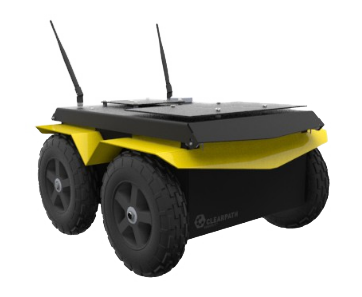
\includegraphics[width=\textwidth]{images/jackal.png}
		\subcaption{Plataforma móvel.}
		\label{fig:pocplat}
	\end{minipage}
	\hfill
	\begin{minipage}[b]{.45\linewidth}
		%		\centering
		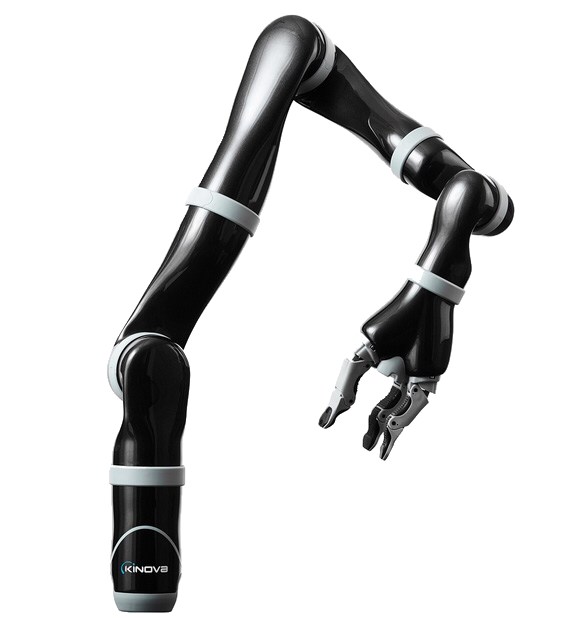
\includegraphics[width=\textwidth]{images/jaco2.png}
		\subcaption{Manipulador.}
		\label{fig:pocmani}
	\end{minipage}
%	\hfill
%	\begin{subfigure}[t]{.3\textwidth}
%		%		\centering
%		\includegraphics[width=\textwidth]{images/whitemarkers.png}
%		\subcaption{Marcadores.}
%		\label{fig:whitemarkers}
%	\end{subfigure}    
	\label{fig:poc}
	\caption{Elementos para a prova de conceito do projeto.}
%	\legend{Fonte: Própria.}
\end{figure}

Dessa forma, esta prova de conceito, subsidiará a análise de viabilidade técnica-econômica prevista para a finalização deste projeto, e que é fundamental para a contratação de futuras fases do projeto.

Além do objetivo principal descrito acima, alguns objetivos específicos devem ser perseguidos para que a conclusão do principal seja alcançada, de forma suscinta é listado estes objetivos específicos:
\begin{itemize}
	\item Projetar e construir a prova de conceito para operação automática de um manipulador 6 \acs{DoF} tendo uma plataforma móvel como referência.
	\item Detalhar operações mais usuais de ROVs e quais manipuladores são utilizados em cada operação.
	\item Elaborar o \textit{\acs{SOTA}} para operação automática de manipuladores submarinos.
	\item Avaliar o custo da operação dos manipuladores e os impactos sobre os custos totais da operação com \acs{ROV}, a partir de referências fornecidas pela PETROBRAS.
	\item Estimar redução nos custos de operação mediante a automatização dos manipuladores, a partir de referências fornecidas pela PETROBRAS.
	\item Elaborar análise de viabilidade técnico-econômica da automatização de operações com manipuladores de \acs{ROV}, a partir de referências fornecidas pela PETROBRAS.
	\item Elaborar um plano de trabalho, considerando que a análise de viabilidade seja positiva, para continuidade do desenvolvimento.
\end{itemize}

No momento atual, alguns desses objetivos já estão sendo desenvolvidos, enquanto outros ainda não foram iniciados; porém espera-se dar início a todos estes objetivos específicos assim que o primeiro workshop seja realizado com o time da Petrobras, que ocorrerá ainda neste mês de maio de 2019.

%---- fase conceitual ------------------------------------
\section{Justificativa}
\label{sec:just}
Nesta etapa da automação de um manipulador, que precede a construção de um protótipo viável em fases futuras, provas de conceito (\textit{\acs{PoC}}) devem ser realizadas em proporções reduzidas em relação às condições reais e em ambiente terrestre, pois acelera o desenvolvimento e possibilita análises de variáveis que podem ser melhor consideradas quando da realização de testes em ambiente controlado. Para isto, algumas abordagens para reproduzir as condições de manipulação subaquática serão testadas demonstrando a aplicação de um ou mais conceitos a partir de diferentes plataformas de desenvolvimento robótico, assim como ferramentas, frameworks, sensores e atuadores que suportem a implementação de técnicas de modelagem de sistemas, controle de posição e de trajetória, integração de sistemas e visão computacional.
A simulação de cenários nas diversas provas de conceitos deverá validar operações que futuramente poderão ser automatizadas por manipuladores subaquáticos em ROVs em intervenções operacionais nas instalações da Petrobrás. 

Um dos pontos importantes na automação de um manipulador robótico é a sua consistência na movimentação de objetos em seu \textit{end-effector}, o fato do desenvolvimento do projeto estar sendo submetido a um ambiente subaquático eleva ainda mais a importância no desenvolvimento de testes conceituais antes da realização do teste final da prova de conceito, onde vários componentes são integrados entre si e desempenham funcionalidades específicas para um ambiente controlado. Trazer estes aspectos para o laboratório é algo que deve ser preponderante para a realização do projeto, pois o mesmo deve ser testado e simulado com elementos capazes de ambientalizar o fenômeno do ponto de visto de controle num ambiente subaquático.

O uso de manipuladores como o sugerido será capaz de trazer à luz do desenvolvimento compreensão sobre as variáveis influenciadoras do evento, utilizados na customização das características técnicas do manipulador robótico a ser testado, os mesmos serão capazes de integrar de forma mais rápida algoritmos a serem desenvolvidos pela equipe do projeto, levando a uma otimização do tempo de desenvolvimento e aumentando a confiabilidade na implementação de controles mais precisos e estáveis.

Dessa forma, a prova de conceito subsidiará a análise de viabilidade técnica-econômica prevista nesta fase, fundamental para a contratação de futuras fases do projeto.

%=========================================================

\section{Organização do relatório}
\label{sec:org}
Este documento está organizado da seguinte forma, o capítulo \ref{chap:int} traz referências iniciais do objetivo deste projeto, o capítulo \ref{chap:robaqua} caracteriza o entendimento sobre a robótica submarina e a atuação dos manipuladores subaquáticos, apresentando de forma suscinta o estado da arte atual para estes elementos, assim como uma pesquisa de anterioridade elaborada para este projeto. O capítulo \ref{chap:manisub-s} descreve a ideia central com relação a prova de conceito que será desenvolvida ao longo deste projeto, chegando a apresentar aspectos iniciais da simulação da prova de conceito. Finalmente, o capítulo \ref{chap:concl} descreve os aspectos conclusivos para esta etapa do projeto.

	\chapter{Robó}
\label{chap:robaqua}
A integridade da infraestrutura offshore é uma questão-chave para a produção ininterrupta de petróleo e gás, bem como para a segurança dos funcionários embarcados. O envelhecimento das infraestruturas causada principalmente pela corrosão e fadiga gera um aumento da probabilidade de falha. Em casos extremos, a perda da integridade estrutural pode causar o colapso da estrutura resultando na perda completa da instalação e ocasionalmente em um desastre ecológico e humano. 

O projeto de vida típico de uma plataforma é de 20 - 25 anos, no entanto, devido à demanda atual para a produção de petróleo e gás, muitas dessas plataformas continuarão em operaçãos além do projetado. A inspeção estrutural da região submersa destas estruturas apresenta um desafio logístico dado o meio subaquático. Logo, a importância do desenvolvimento de sistemas submarinos adequados para inspeções periódicas de integridade estrutural. Um agravante a este problema é o aumento do percentual da produção executada por equipamento submersos, que resulta em uma maior demanda de inspeção periódica dos equipamentos posicionados no fundo marinho.  

Atualmente, as estruturas subaquáticas são inspecionados ou por ROVs ou mergulhadores. Ambos os métodos são dispendiosos e ineficientes, principalmente por duas razões: 
\begin{itemize}
	\item necessidade de pessoal altamente especializado;
	\item e o tempo necessário para realizar inspeções manualmente.
\end{itemize}

Portanto, o principal desafio no problema de inspeção estrutural submarina reside no desenvolvimento de um método eficiente de inspeção, que não necessita de um pessoal altamente especializado e que pode ser utilizada diretamente a partir das plataformas, sem a necessidade de uma embarcação de suporte.  


%\section{Veículos de operação remota}
%\label{chap:sotarov}
%
%\subsection{Estudo do estado da arte}
%\label{sec:sotarov}
%pybullet
%\subsubsection{Benchmarking}
%\label{ssec:benchrov}
%
%\subsubsection{Estudo de comparação das operações de ROV}
%\label{sec:comprov}
%
%\ldots

%------------------------------------------------------------

\section{Manipuladores subaquáticos}
\label{chap:sotamani}



Um manipulador, também conhecido com um braço robótico, é considerado a ferramenta mais adequada para executar operações de intervenção submarina. Assim, os veículos submarinos não tripulados (\textit{\acs{UUV}s}), como os veículos operados remotamente (ROVs) e, em alguns casos, os veículos subaquáticos autônomos (\textit{\acs{AUV}s}) são equipados com um ou mais manipuladores submarinos. UUVs com manipuladores são freqüentemente chamados de Manipulador de Veículos Subaquáticos (\textit{\acs{UVM}s}). Segundo \cite{sivvcev2018underwater}, a maioria dos manipuladores subaquáticos existentes usados ​​nos UUVs são antropomórficos, ou seja, eles são projetados para se assemelhar a um braço humano. Esses manipuladores são compostos de uma seqüência de corpos rígidos (links) interconectados por meio de juntas rotacionais com um deslocamento angular adequado entre elas e garras ou outras ferramentas intercambiáveis ​​presas no \textit{end-effector}. Para a observação de seu entorno, eles são geralmente acompanhados por um equipamento adicional composto por uma ou mais câmeras e holofotes montados no veículo subaquático da base e/ou no próprio manipulador.

Os manipuladores subaquáticos são usados ​​para uma variedade de tarefas submarinas em diferentes aplicações em petróleo e gás offshore, energia renovável e indústrias de engenharia civil marinha, bem como em ciências marinhas e aplicações militares \cite{capocci2017inspection}. Como eles estão sendo usados ​​em uma ampla gama de aplicações, os manipuladores submarinos são projetados para diferentes propósitos, por ex. existem manipuladores com mobilidade limitada equipados com garras para içar objetos grandes e pesados, manipuladores usados ​​para fixar uma garra destacável a um objeto afundado selecionado, manipuladores de garras equipados com garras ou copos de vácuo usados ​​para fixar um veículo submerso a estruturas submersas ou perto de paredes planas durante a operação, manipuladores equipados com dispositivos de inspeção, manipuladores de intervenção hábeis com garras que podem transportar diferentes ferramentas usadas para operações de reparo e manutenção em estruturas submersas etc. Geralmente, os ROVs da classe trabalhadora são equipados com dois manipuladores, na maioria dos casos simples agarrador poderoso para segurar o ROV perto da estrutura de engenharia hidráulica ou naufrágio, enquanto o outro manipulador realiza a tarefa de intervenção real.

Algumas das tarefas que os manipuladores subaquáticos são projetados para executar incluem inspeção de tubos \cite{christ2013rov}, salvamento de objetos afundados \cite{chang2004distance}, limpeza de superfícies \cite{davey1999non}, abertura e fechamento de válvulas, perfuração, corte de cabos \cite{christ2013rov}, assentamento e reparo de cabos, limpeza de entulhos e redes de pesca, biológica \cite{jones2009using} e amostragem geológica \cite{noe2006surface}, etc. Em geral, os manipuladores estão localizados na parte frontal do veículo submerso, mas nem sempre é esse o caso, por exemplo, há veículos com um manipulador localizado na parte inferior lado \cite{ribas2011girona}.

\subsection{Estudo do estado da arte}
\label{sec:sotamani}
De forma abrangente o estado da arte do conhecimento sobre os sistemas manipuladores subaquáticos foi baseado inicialmente em um artigo fundamentado por \citeonline{sivvcev2018underwater}. 

Os autores forneceram uma pesquisa sobre o uso da tecnologia de manipulação para uma variedade de operações de intervenção submarina e inspeção em diferentes áreas de aplicação offshore. Ambas as soluções de manipuladores subaquáticos comercialmente disponíveis e os sistemas de protótipos foram analisados. Tópicos relevantes foram discutidos, incluindo especificações técnicas de manipuladores, projeto mecânico, atuação, modelagem de robô (cinemática e dinâmica), abordagens de controle e algoritmos (controle de movimento, controle cinemático, planejamento de movimento) e uma comparação detalhada foi apresentada destacando vantagens e desvantagens de diferentes soluções presentes na tecnologia de manipulação submarina. Este tópico apresenta uma imagem atual da tecnologia existente a fim de fornecer uma fonte útil para futuras pesquisas no campo da robótica subaquática e manipulação. Fatores críticos que limitam o desempenho de manipuladores subaquáticos passaram a ser mais entendidos a partir da revisão abrangente deste estado da arte. Os autores recomendam fortemente que esses fatores sejam considerados durante o projeto de futuros sistemas manipuladores subaquáticos.

%fazer um mapa mental sobre os tópicos relevantes

Muitos pesquisadores \cite{wang2008novel} \cite{suboh2009modeling} \cite{golea2002fuzzy} \cite{pandian2010neuro} têm trabalhado no desenvolvimento de algoritmos de controle, mas poucos foram implementados e testados em sistemas de manipuladores submarinos físicos. 
Além disso, não há manipuladores comerciais controláveis ​​por torque no momento. Portanto, muitos dos algoritmos de controle de baixo nível propostos não são aplicáveis ​​a sistemas comerciais e até mesmo à maioria dos protótipos. Pesquisas acadêmicas relativamente recentes que incluiam ensaios submarinos experimentais em ambiente de campo ou pelo menos em tanques de teste tem sido realizada na Ocean One, MARIS, TRIDENT, RAUVI, PANDORA, CManipulator e KORDI. 
Os dois últimos tem concentrado suas pesquisas em sistemas de manipuladores de ROV hidráulicos comerciais, enquanto os restantes concentram nas intervenções de AUVs com manipuladores de protótipos elétricos. 
Alguns dos projetos em curso na atualidade estão sendo desenvolvidos em ambientes relevantes de manipulação submarina, desta forma pode-se estabelecer uma pequena lista:
%as empresas precisam ser referenciadas ou nota de rodapé
\begin{itemize}
	\item ROBUST \url{http://eu-robust.eu/};
	\item MERBOTS \url{http://www.irs.uji.es/project/merbots}; 
	\item DexROV \url{http://www.dexrov.eu/};
	\item Operations Support Engineering - MaREI \url{http://www.mmrrc.ul.ie/};
\end{itemize}
 
Destes projetos acima, a Operation Support Engineering - MaREI faz uso de manipuladores hidráulicos padrão da indústria em ROV, e o restante usa manipuladores elétricos em AUVs.

Uma visão introdutória como a apresentada acima, pode dirimir inicialmente sobre o tema de forma macro, porém para uma pesquisa mais profunda há que se levar em consideração subtópicos para que temas mais profundos possam ser estudados. Neste sentido o projeto toma como referência a divisão apresentada por \citeonline{sivvcev2018underwater} com algumas modificações em sua separação (fFigura \ref{fig:estrusub}).
 
%preparar figura dos tópicos relevantes
%------ picture -------------
%\begin{sidewaysfigure*}
\begin{figure}[H] 
  \begin{center} 
  	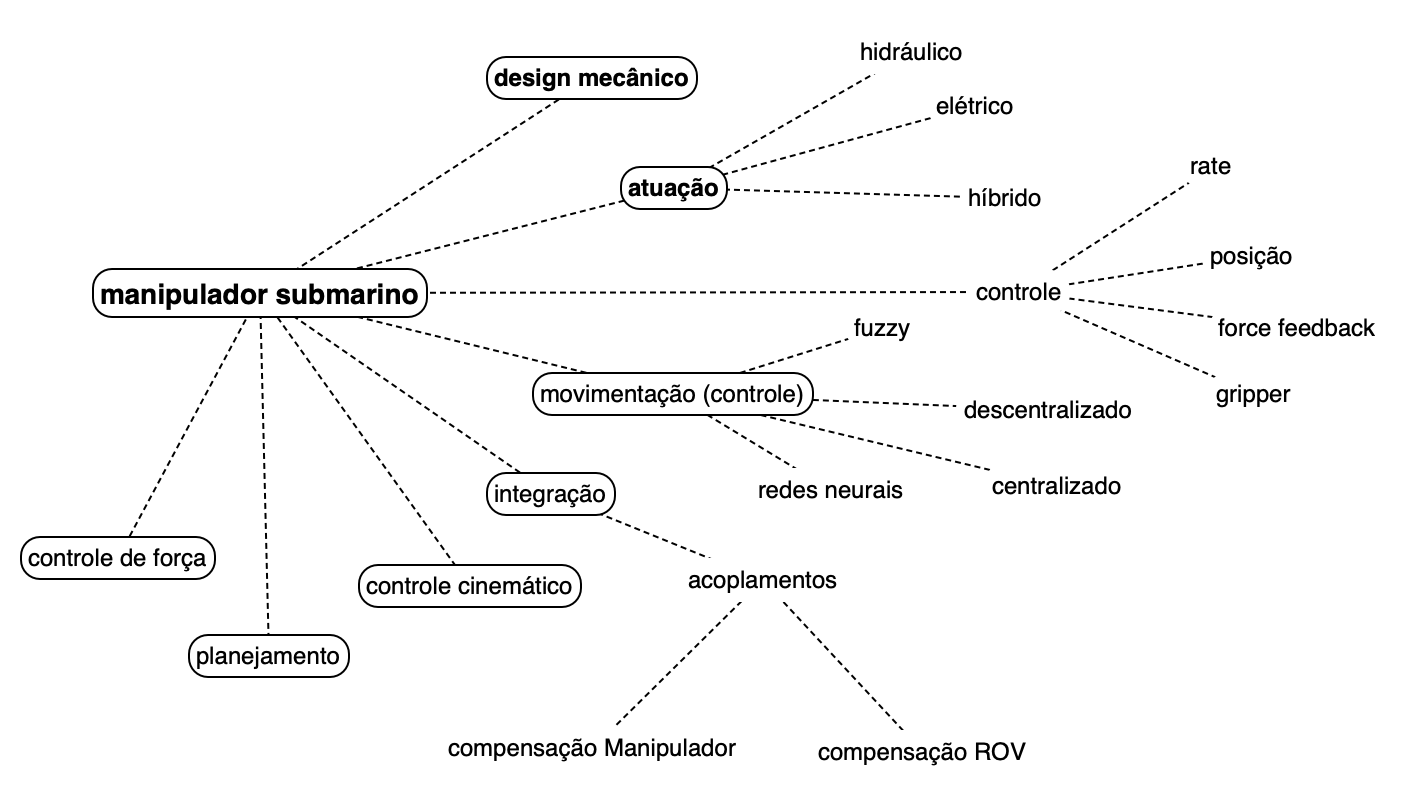
\includegraphics[width=0.9 \textwidth]{images/manipuladorsubmarino.png} 
  \end{center} 
  \caption{Estrutura de subsistemas para um manipulador submarino.} 
  %\legend{Fonte: os autores.} 
  \label{fig:estrusub} 
\end{figure}
%\end{sidewaysfigure*}
%----------------------------

\subsubsection{Design mecânico}
\label{sec:desmeca}

Os materiais mais comuns usados ​​na construção de manipuladores subaquáticos são ligas de metal, muitas vezes escolhidos por causa da alta resistência do material e propriedades contra corrosão. Com o objetivo de reduzir o peso na água e aliviar a carga dispendida pelo atuador experimentos tem sido desenvolvidos para incrementar capacidade de flutuabilidade nos manipuladores \cite{ishimi1991manipulation}.

Normalmente os manipuladores submarinos mais robustos são concebidos para atuar entre 3000 a 6500 metros da água do mar, no entanto alguns manipuladores foram desenvolvidos podendo atingir até 7000m, como é o caso do manipulador da Schilling Robotics - Titan 4 e um protótipo desenvolvido por \citeonline{zhang20147000m}.

Além disso, existem alguns sistemas projetados para a profundidade total do oceano, ou seja 11.000 metros de profundidade. O Instituto Oceanográfico Woods Hole, em colaboração com a Kraft Robotics, projetou um desses manipuladores para o propósito da missão de exploração da Mariana Trench \cite{bowen2008nereus}. Outros incluem "Magnum 7", um produto da ISE Ltd. e "The ARM" e "MK-37", desenvolvidos pela Western Space and Marine, Inc.

O tamanho dos manipuladores subaquáticos é descrito por um parâmetro chamado "Reach" que representa o comprimento de toda a cadeia cinemática do manipulador. Juntamente com a amplitude de movimento das articulações, determina o tamanho da área de trabalho do manipulador, um conjunto de pontos que podem ser alcançados pelo seu efeito final \cite{cao2011accurate}. O alcance dos manipuladores subaquáticos existentes varia de 0,5 m para os manipuladores de garras até 2,4 m para manipuladores mais robustos.

O torque máximo do punho que os manipuladores subaquáticos são capazes de produzir varia de 8Nm a 250Nm. De acordo com a ISO 13628–8:2010 \cite{iso2010petroleum}, as interfaces ROV rotativas de baixo torque em sistemas de produção submarina, que normalmente são usadas em válvulas de agulha submarinas, têm classificação máxima de 75Nm. Além disso, a capacidade de elevação de carga dos manipuladores submarinos varia de 5 kg a 500 kg. Os fabricantes costumam fornecer parâmetros diferentes para a capacidade de elevação do manipulador; o que torna a comparação não trivial, pois a capacidade de carga não é uma valor fixo, mas depende da posição do manipulador.

Em geral, o peso de um manipulador submarino não molhado está entre 6 kg e 150 kg; no entanto, seu peso na água é mais importante pois determina a flutuabilidade necessária no veículo de base para compensar o manipulador. O peso e o tamanho são fatores muito importantes, pois são diretamente responsáveis ​​pela quantidade de acoplamento dinâmico introduzido entre o manipulador e o robô submarino no qual está montado e, portanto, pode influenciar o desempenho de todo o sistema. 

Para poder explorar completamente as características do manipulador, o peso do manipulador deve ser uma porcentagem baixa o suficiente, para que o acoplamento dinâmico possa ser desprezado ou pelo menos levado em consideração como uma perturbação externa que pode ser tratado pelo posicionamento dinâmico do robô submarino (ROV). 

Maior peso e tamanho maior geram demandas mais altas com relação à robustez do sistema de propulsão de um robô submarino (ROV) quando submetido às perturbações causadas pelo acoplamento dinâmico. 

 A Tabela 2 apresenta o peso relativo do manipulador para o veículo para os ROVs comerciais pesados, médios e leves da classe comercial. Pode-se observar que essa relação é significativamente baixa, mesmo para os veículos comerciais leves da classe trabalhadora.

%tabela dos rovs com os manipuladores

Os manipuladores subaquáticos podem ser equipados com vários tipos de pinças no seu \textit{end effector}. As soluções comerciais apresentam diferentes garras intercambiáveis, cada uma com seu objetivo específico. Um tipo de garra comum é aquele com garras de ação paralela, que inclui um \textit{slot} para uma alça de barra T padrão \cite{iso2010petroleum}, e sua função principal é agarrar diferentes objetos e ferramentas em uma variedade de operações submarinas. As ferramentas geralmente são projetadas com uma barra em T exatamente para esse fim. As garras diferentes incluem garras de três ou quatro dedos, garras flutuantes de dois ou três dedos, garras de tesoura, pés de sucção, etc. Os atuadores das garras são geralmente hidráulicos e a força de garra das garras disponíveis comercialmente variam de 35 kgf a 652 kgf.

Dependendo da natureza da tarefa para a qual foram projetados, os manipuladores subaquáticos vêm com diferentes números de graus de liberdade (DOF). Os manipuladores subaquáticos comerciais e experimentais são geralmente projetados com três a seis DOFs, sem levar em consideração a mobilidade da garra. A razão para isso é que três DOFs são suficientes para alcançar uma posição arbitrária e seis DOFs para posição arbitrária e orientação do \textit{end effector} na área de trabalho \cite{spong2005robot}. 
O termo “função n” é frequentemente usado na literatura para descrever o número de atuadores contidos em um manipulador e esse termo também inclui a mobilidade da garra, portanto, por exemplo, um manipulador de sete funções significa que existem seis atuadores responsável pelo movimento do manipulador que fornece seis DOFs verdadeiros mais um atuador para a mobilidade da garra. Manipuladores subaquáticos com sete ou mais DOFs (sem mobilidade da pinça) não são muito comuns, mas existem. 

Manipuladores com 7 DOF são inerentemente redundantes do ponto de vista cinemático \cite{siciliano2010robotics}. Esse recurso pode desempenhar um papel importante na autonomia de manipuladores, pois a redundância pode ser explorada para um objetivo secundário, tal como evitar obstáculos. 

Manipuladores submarinos com 7 DOF é relatada por \citeonline{marani2009underwater} e \citeonline{ribas2015auv} e com oito DOF por \citeonline{greig1994arm}. 

Qualquer aplicação robótica de manipuladores subaquáticos requer algoritmos de planejamento e controle de modelagem cinemáticos aplicáveis. Os manipuladores subaquáticos geralmente têm estrutura mecânica de cadeia serial semelhante aos braços de manipuladores industriais. Existe muita literatura sobre a cinemática de robôs que pode ser aplicada a manipuladores subaquáticos, alguns dos quais podem ser encontrados em \citeonline{spong2005robot}; \citeonline{siciliano2010robotics}; e \citeonline{corke2011robotics}. 

Literatura adicional sobre sistemas manipuladores de veículos pode ser encontrada em \citeonline{p2014vehicle} e literatura mais específica relacionada a sistemas manipuladores de veículos subaquáticos em \citeonline{antonelli2014unrob}.

%inserir a tabele 1

\subsubsection{Atuação}
\label{sec:atua}
Na atualidade há dois caminhos importantes identificados no desenvolvimento de manipuladores submarinos, ambos apresentam vantagens e desvantagens, são eles: um baseado em óleo hidráulico e outro em atuadores elétricos. Há ainda algumas ideias apresentadas como uma combinação entre ambos, conforme apresentado por \citeonline{denket2006frontiers}.

Na grande maioria, os manipuladores baseados em óleo hidráulico são os mais tipicamente usados, mesmo assim há muitos pontos a serem considerados como novas perspectivas para o desenvolvimento de novas características, tanto \citeonline{yao2009development}, \citeonline{zhang20147000m} como \citeonline{zuyao2011design} apresentam em suas pesquisas novas características e configurações.

As soluções baseadas na perspectiva dos atuadores elétricos são menores do que a vertente anterior além de que alguns requisitos tais como velocidade, confiabilidade ou força podem não atender a certos requisitos para uma determinada intervenção, porém apresentam um campo ainda pouco explorado; capacidade de controle preciso nos movimentos e possibilidade de controle de torque são as vantagens principais para este tipo de manipuladores \cite{ribas2015auv} \cite{fernandez2013grasping}.


%\subsection{Sistema de controle}
%\label{sec:siscon}
%
%\subsection{Controle de movimentação}
%\label{sec:conmovi}
%
%\subsection{Integração}
%\label{sec:integ}
%
%\subsection{Planejamento da movimentação}
%\label{sec:plan}
%
%\subsection{Controle de força}
%\label{sec:conforce}
%
%\subsection{Controle da Cinemática}
%\label{sec:conkine}

\subsection{Pesquisa de anterioridade}
\label{sec:pesant}
A pesquisa de anterioridade realizada neste início de projeto tem como o principal objetivo verificar diante da base de conhecimento nacional e internacional a disponibilidade de ideias e patentes desenvolvidas sob o mesmo ambiente do projeto. A busca teve como ponto de partida desenvolvimentos que tinham como base manipuladores de 6DoF e que possuíam tomada de decisão autônoma. As palavras chaves determinadas para a pesquisa foram: 
\begin{itemize}
	\item Manipulação subaquática
	\item Manipulador subaquático
	\item Manipulador subaquático autônomo
	\item Braço robótico subaquático
	\item Braço robótico subaquático autônomo
	\item Robótica submarina
	\item ROV
	\item Veículo Operado Remotamente
	\item Controle de manipuladores subaquático
\end{itemize}
	
As bases de procura utilizadas para a formação do relatório de anterioridade foram:
\begin{itemize}
	\item INPI – Instituto Nacional de Propriedade Industrial 	\url{www.inpi.gov.br}
	\item  ESPACENET – European Patent Office 	\url{pt.espacenet.com}
	\item USPTO – United States Patent and Trademark Office \url{	www.uspto.gov}
	\item SCIELO – Scientific Eletronic Library on line \url{	www.scielo.com.br}
	\item Portal de Periódicos da CAPES	\url{www.periodicos.capes.gov.br}
	\item WIPO – Organização Mundial de Propriedade Intelectual 	\url{www.wipo.int}
	\item Google patents	 \url{www.google.com/patents}
	\item Clarivate Analytics - Derwent Innovation	\url{www.derwentinnovation.com}
\end{itemize}

O resultado da busca, realizada num espaço que compreende entre 2000 e 2018, encontrou 39 patentes centradas na temática MANIPULADOR SUBAQUÁTICO AUTÔNOMO, entanto 21 delas tem uma maior relevância e podem ser melhor analisadas no Anexo \ref{ann:relant} .

Um ponto a ser observado também é a origem destas patentes, abaixo a Figura \ref{fig:relpat} apresenta as empresas que mais depositaram patentes sobre o assunto, sendo: 
\begin{enumerate}
	\item TESCO CORP.
	\item EELUME AS.
	\item MITSUBISHI HEAVY INDUSTRIES LTD.
	\item SAMSUNG HEAVY INDUSTRIES LTD.
	\item UNIV NORTHEAST PETROLEUM
	\item UNIVERSITY OF WASHINGTON
	\item OCEANEERING INTERNATIONAL INC.
	\item KOREA ADVANCED INSTITUTE FOR SCIENCE AND TECHNOLOGY
	\item MOTORWEL CO LTD.
	\item NORWEGIAN UNIV OF SCIENCE \& TECHNOLOGY (NTNU)
\end{enumerate}

%------ picture -------------
%\begin{sidewaysfigure*}
\begin{figure}[H] 
  \begin{center} 
  	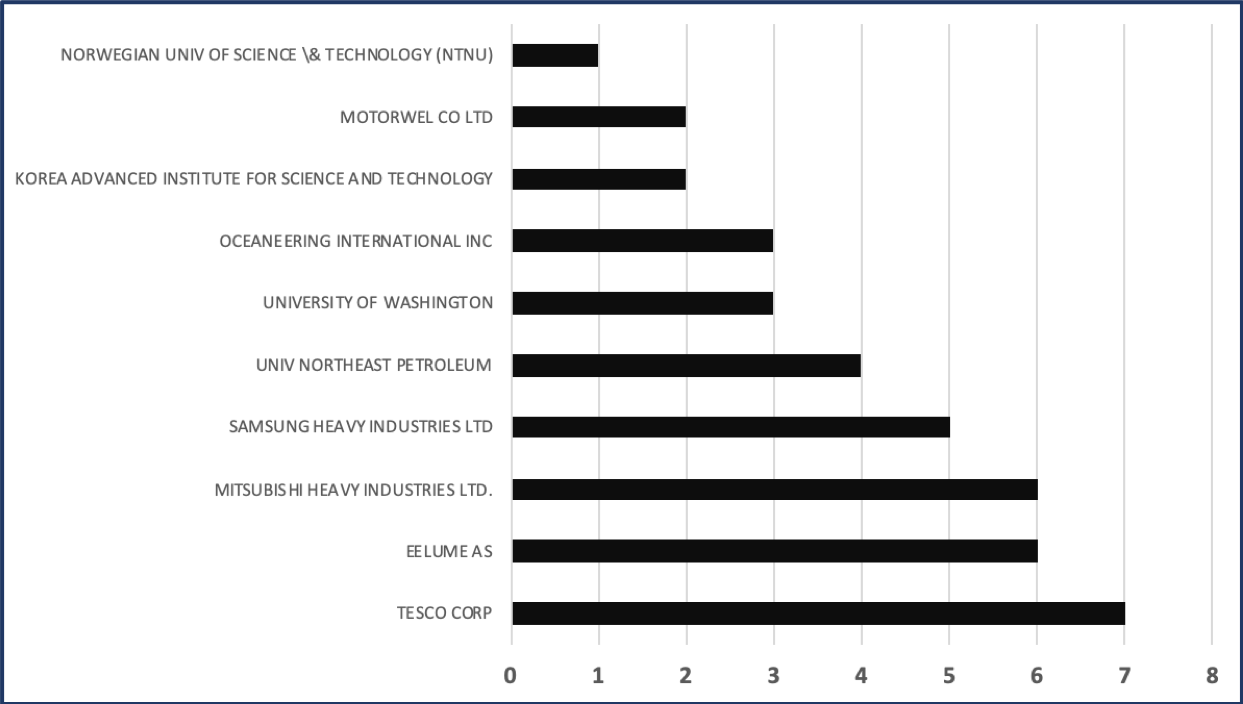
\includegraphics[width=0.9 \textwidth]{images/patenteslist.png} 
  \end{center} 
  \caption{Relação de patentes.} 
  %\legend{Fonte: os autores.} 
  \label{fig:relpat} 
\end{figure}
%\end{sidewaysfigure*}
%----------------------------

% \begin{tikzpicture}
% 	\begin{axis}[title  = Contributions per category
% 							at LaTeX-Community.org,
% 	  xbar,
% 	  y axis line style = { opacity = 0 },
% 	  axis x line       = none,
% 	  tickwidth         = 0pt,
% 	  enlarge y limits  = 0.2,
% 	  enlarge x limits  = 0.02,
% 	  symbolic y coords = {LaTeX, Tools, Distributions, Editors},
% 	  nodes near coords,
% 	]
% 	\addplot coordinates { (57727,LaTeX)         (5672,Tools)
% 						   (2193,Distributions)  (11106,Editors) };
% 	\addplot coordinates { (14320,LaTeX)         (1615,Tools)
% 						   (560,Distributions)   (3075,Editors)  };
% 	\legend{Topics, Posts}
% 	\end{axis}
%   \end{tikzpicture}

A Coréia é o país com maior número de patentes (11 registros), em seguida vem os EUA com 9 registros e a China com 3 patentes.
O relatório apresenta ainda um fato interessante que a grande maioria das patentes encontradas tiveram o seu depótiso no ano de 2017, totalizando em torno de 11 patentes submetidas e registaradas.

A busca também levou em consideração a identificação de artigos científicos relevantes para a pesquisa, os mais relevantes são:  
\begin{itemize}
	\item Research on Underwater Safety Inspection and Operational Robot Motion Control \cite{guangyi2018research};
	\item Augmented reality visualization of scene depth for aiding ROV pilots in underwater manipulation \cite{bruno2018augmented};
	\item Dynamic Modeling and Identification of an Heterogeneously Actuated Underwater Manipulator Arm \cite{leborne2018dynamic};
	\item Design, prototyping and testing of a modular small-sized underwater robotic arm controlled through a Master-Slave approach \cite{barbieri2018design};
	\item Underwater manipulators: A review \cite{sivvcev2018underwater};
	\item A Modular Soft Robotic Wrist for Underwater Manipulation \cite{kurumaya2018modular};
	\item Fully automatic visual servoing control for work-class marine intervention ROVs \cite{sivvcev2018fully};
	\item Collision Detection for Underwater ROV Manipulator Systems \cite{sivvcev2018collision};
	\item Kinematic performances evaluation of a hydraulic underwater manipulator \cite{rizzo2017kinematic};
	\item Impact of Arm Morphology on the Hydrodynamic Behavior of a Two-arm Robotic Marine Vehicle \cite{kazakidi2017impact};
	\item Development of Hand Gesture Recognition Sensor Based on Accelerometer and Gyroscope for Controlling Arm of Underwater Remotely Operated Robot \cite{mardiyanto2017development};
	\item Robust Adaptive PID Control for Positioning of Remotely Operated Vehicle Working in Close Proximity of an Underwater Structure \cite{qiao2016robust};
	\item Development of a Virtual Platform for Telepresence Control of an Underwater Manipulator Mounted on a Submersible Vehicle \cite{zhang2016development};
	\item The Underwater Swimming Manipulator - A Bio-Inspired AUV \cite{sverdrup2016underwater};
	\item Convolutional Neural Network-based Real-time ROV Detection Using Forward-looking Sonar Image \cite{kim2016convolutional};
	\item I-AUV Docking and Panel Intervention at Sea \cite{palomeras2016auv};
	\item 3D-Belief Space Planning for underwater mobile \cite{zereik20153d};
	\item Intervention AUVs: The next challenge \cite{ridao2014intervention};
	\item Rotation Identification in Geometric Algebra: Theory and Application to the Navigation of Underwater Robots in the Field \cite{stanway2015rotation};
	\item I-AUV Docking and Intervention in a Subsea Panel \cite{palomeras2014auv};
	\item Design of Modular Camera Tool for Mini Underwater ROVs \cite{poretti2013design};
	\item Design of a gateway for remotely underwater vehicles \cite{liu2012design};
	\item Stochastic controllers for robust underwater mobile manipulation \cite{bonsignorio2012stochastic};
	\item New Approach for a Reconfigurable Autonomous Underwater Vehicle for Intervention \cite{de2009new};
	\item Manipulability analysis of underwater robotic arms on ROV and application to task-oriented joint configuration \cite{jun2004manipulability};
	\item ArmillEye: Flexible platform for underwater stereo vision \cite{zoppi2007armilleye};
	\item Adaptive PD-controller for positioning of a remotely operated vehicle close to an underwater structure: Theory and experiments \cite{hoang2007adaptive};
	\item A composite rigid body algorithm for modeling and simulation of an underwater vehicle equipped with manipulator arms \cite{hosseini2006composite};
	\item Navigation and control system of a deep-sea unmanned underwater vehicle 'HEMIRE' \cite{lee2007navigation};
	\item Manipulability analysis of underwater robotic arms on ROV and application to task-oriented joint configuration \cite{jun2004manipulability};
	\item A fuzzy approach to redundancy resolution for underwater vehicle-manipulator systems \cite{antonelli2000fuzzy};
	\item Controlling an uninstrumented manipulator by visual servoing \cite{marchand2002controlling};
	\item Control architecture and operator interface for a free-flying robotic vehicle \cite{carignan2001control};
	\item Controlling an uninstrumented ROV manipulator by visual servoing \cite{marchand2001controlling};
	\item Controlling the manipulator of an underwater ROV using a coarse calibrated pan/tilt camera \cite{marchand2001controllingx};
	\item Forestry equipment strikes fear into trees \cite{heney2000features};
	\item Control laws, tasks and procedures with ORCCAD: application to the control of an underwater arm \cite{simon1998control};
	\item Hybrid position/force control of a ROV with a manipulator \cite{lapierre1998hybrid};
	\item A virtual environment for undersea telepresence \cite{schebor1995virtual};
	\item Subsea weld inspection using an advanced robotic manipulator \cite{broome1995subsea};
	\item Experiments in the coordination of underwater manipulator and vehicle control \cite{mclain1995experiments};
	\item Concept evaluation trials of teleoperation system for control of an underwater robotic arm by graphical simulation techniques \cite{boyle1995concept};
	\item Advanced controller for an underwater manipulator \cite{larkum1994advanced};
	\item Planning and control for coordination of underwater manipulators \cite{lane1991planning};
\end{itemize}


%\subsubsection{Benchmarking}
%\label{ssec:benchmani}
%
%\subsubsection{Estudo de comparação das operações de ROV}
%\label{sec:compmani}



\ldots







	%\chapter{r}
A integridade da infraestrutura offshore é uma questão-chave para a produção ininterrupta de petróleo e gás, bem como para a segurança dos funcionários embarcados. O envelhecimento das infraestruturas causada principalmente pela corrosão e fadiga gera um aumento da probabilidade de falha. Em casos extremos, a perda da integridade estrutural pode causar o colapso da estrutura resultando na perda completa da instalação e ocasionalmente em um desastre ecológico e humano.

O projeto de vida típico de uma plataforma é de 20 - 25 anos, no entanto, devido à demanda atual para a produção de petróleo e gás, muitas dessas plataformas continuarão em operaçãos além do projetado. A inspeção estrutural da região submersa destas estruturas apresenta um desafio logístico dado o meio subaquático. Logo, a importância do desenvolvimento de sistemas submarinos adequados para inspeções periódicas de integridade estrutural. Um agravante a este problema é o aumento do percentual da produção executada por equipamento submersos, que resulta em uma maior demanda de inspeção periódica dos equipamentos posicionados no fundo marinho.

Atualmente, as estruturas subaquáticas são inspecionados ou por ROVs ou mergulhadores. Ambos os métodos são dispendiosos e ineficientes, principalmente por duas razões:

\begin{itemize}
	\item necessidade de pessoal altamente especializado;
	\item e o tempo necessário para realizar inspeções manualmente.
\end{itemize}

Portanto, o principal desafio no problema de inspeção estrutural submarina reside no desenvolvimento de um método eficiente de inspeção, que não necessita de um pessoal altamente especializado e que pode ser utilizada diretamente a partir das plataformas, sem a necessidade de uma embarcação de suporte.

\section{Manipuladores subaquáticos}
\label{chap:sotamani}
Um manipulador, também conhecido com um braço robótico, é considerado a ferramenta mais adequada para executar operações de intervenção submarina. Assim, os veículos submarinos não tripulados (\textit{\acs{UUV}s}), como os veículos operados remotamente (ROVs) e, em alguns casos, os veículos subaquáticos autônomos (\textit{\acs{AUV}s}) são equipados com um ou mais manipuladores submarinos. UUVs com manipuladores são freqüentemente chamados de Manipulador de Veículos Subaquáticos (\textit{\acs{UVM}s}).

% Segundo \cite{sivvcev2018underwater}

% Algumas das tarefas que os manipuladores subaquáticos são projetados para executar incluem inspeção de tubos \cite{christ2013rov}, salvamento de objetos afundados \cite{chang2004distance}, limpeza de superfícies \cite{davey1999non}, abertura e fechamento de válvulas, perfuração, corte de cabos \cite{christ2013rov}, assentamento e reparo de cabos, limpeza de entulhos e redes de pesca, biológica \cite{jones2009using} e amostragem geológica \cite{noe2006surface}, etc. Em geral, os manipuladores estão localizados na parte frontal do veículo submerso, mas nem sempre é esse o caso, por exemplo, há veículos com um manipulador localizado na parte inferior lado \cite{ribas2011girona}.

\subsection{Estudo do estado da arte}
\label{sec:sotamani}
De forma abrangente o estado da arte do conhecimento sobre os sistemas manipuladores subaquáticos foi baseado inicialmente em um artigo fundamentado por

%\citeonline{sivvcev2018underwater}.
Os autores forneceram uma pesquisa sobre o uso da tecnologia de manipulação para uma variedade de operações de intervenção submarina e inspeção em diferentes áreas de aplicação offshore. Ambas as soluções de manipuladores subaquáticos comercialmente disponíveis e os sistemas de protótipos foram analisados. Tópicos relevantes foram discutidos, incluindo especificações técnicas de manipuladores, projeto mecânico, atuação, modelagem de robô (cinemática e dinâmica), abordagens de controle e algoritmos (controle de movimento, controle cinemático, planejamento de movimento) e uma comparação detalhada foi apresentada destacando vantagens e desvantagens de diferentes soluções presentes na tecnologia de manipulação submarina. Este tópico apresenta uma imagem atual da tecnologia existente a fim de fornecer uma fonte útil para futuras pesquisas no campo da robótica subaquática e manipulação. Fatores críticos que limitam o desempenho de manipuladores subaquáticos passaram a ser mais entendidos a partir da revisão abrangente deste estado da arte. Os autores recomendam fortemente que esses fatores sejam considerados durante o projeto de futuros sistemas manipuladores subaquáticos.
Além disso, não há manipuladores comerciais controláveis ​​por torque no momento. Portanto, muitos dos algoritmos de controle de baixo nível propostos não são aplicáveis ​​a sistemas comerciais e até mesmo à maioria dos protótipos. Pesquisas acadêmicas relativamente recentes que incluiam ensaios submarinos experimentais em ambiente de campo ou pelo menos em tanques de teste tem sido realizada na Ocean One, MARIS, TRIDENT, RAUVI, PANDORA, CManipulator e KORDI.
Os dois últimos tem concentrado suas pesquisas em sistemas de manipuladores de ROV hidráulicos comerciais, enquanto os restantes concentram nas intervenções de AUVs com manipuladores de protótipos elétricos.
Alguns dos projetos em curso na atualidade estão sendo desenvolvidos em ambientes relevantes de manipulação submarina, desta forma pode-se estabelecer uma pequena lista:
\begin{itemize}
	\item ROBUST \url{http://eu-robust.eu/};
	\item MERBOTS \url{http://www.irs.uji.es/project/merbots}; 
	\item DexROV \url{http://www.dexrov.eu/};
	\item Operations Support Engineering - MaREI \url{http://www.mmrrc.ul.ie/};
\end{itemize}
	%=========================================================
%---- fase conceitual ------------------------------------
%=========================================================
%\chapter{BASIS OF DESIGN}
%\label{chap:bod}
%
%%---- fase conceitual ------------------------------------
%\section{Requisitos do cliente}
%\label{sec:reqcli}
%
%%---- fase conceitual ------------------------------------
%\section{Estudo do estado da arte}
%\label{sec:sota}
%
%%---- fase conceitual ------------------------------------
%\subsection{Benchmarking}
%\label{sec:bnchmkg}
%
%%---- fase conceitual ------------------------------------
%\section{Ambiente de operação}
%\label{sec:ambopt}
%
%%---- fase conceitual ------------------------------------
%\section{Normas}
%\label{sec:normas}


\chapter{MANIPULADOR SUBAQUÁTICO - \textit{PoC}}
\label{chap:manisub-s}
Este capítulo tem o objetivo de apresentar a concepção do desenvolvimento de várias funcionalidades de um manipulador subaquático e que seja capaz de reconhecer alvos e consequentemente realizar tarefas de forma autônoma, mesmo que seu frame de localização seja alterado durante a missão. É importante salientar que o desenvolvimento deste projeto procura estabelecer uma prova de conceito para que estas funcionalidades sejam testadas mesmo antes de um envolvimento num ambiente subaquático.

As funcionalidades a serem testadas em laboratório são: 
\begin{enumerate}
	\item percepção do manipulador: esta funcionalidade tem por objetivo reconhecer um marcador tipo \textit{aprilTag} (Figura \ref{fig:apriltag}) e identificar a posição de atuação para a trajetória da missão.
	\item navegação da plataforma móvel: objetivo é fornecer comandos para realização de movimentos tanto em manual com em rotas pré-programadas, nestas rotas pontos aleatórios serão gerados simulando distúrbios marinhos que podem ocorrem em ROVs.
	\item planejamento da trajetória: diante da informação da posição a ser realizada e tendo as perturbações geradas, o planejamento será capaz de reposicionar o \textit{end-effector} do manipulador para atender a trajetória do mesmo.
	\item atuação do manipulador: o objetivo principal desta funcionalidade será o de realizar o comando de apertar o botão localizado pela primeira funcionalidade abordada.
\end{enumerate}

%------ picture -------------
%\begin{sidewaysfigure*}
\begin{figure}[H] 
  \begin{center} 
  	
\includegraphics[width=0.4 \textwidth]{images/apriltag.png} 
  \end{center} 
  \caption{Exemplo de um marco fiducial (apriltag).} 
  %\legend{Fonte: os autores.} 
  \label{fig:apriltag} 
\end{figure}
%\end{sidewaysfigure*}
%----------------------------



%\section{Base of design}
\section{Base do desenvolvimento}
\label{sec:bod-s}
Um dos pontos importantes para uma pesquisa inicial de uma determinada tecnologia, é poder testar alguns funcionalidades da ideia principal com um mínimo de recursos necessários para o desenvolvimento de um protótipo. Neste projeto para testar várias das funcionlidades apresentadas na introdução do capítulo \ref{chap:manisub-s}, foi considerado analogamente dois elementos para simular tanto o ROV quanto o manipulador subaquático. Para simular as perturbações do ambiente aquático, foi idealizado desenvolver a PoC num piso irregular, que pudesse a todo tempo alterar o psocionamento da base do manipulador.

De forma descritiva, a Figura \ref{fig:manipoc} apresenta uma ideia sobre o teste a ser realizado

%------ picture -------------
%\begin{sidewaysfigure*}
\begin{figure}[H] 
  \begin{center} 
  	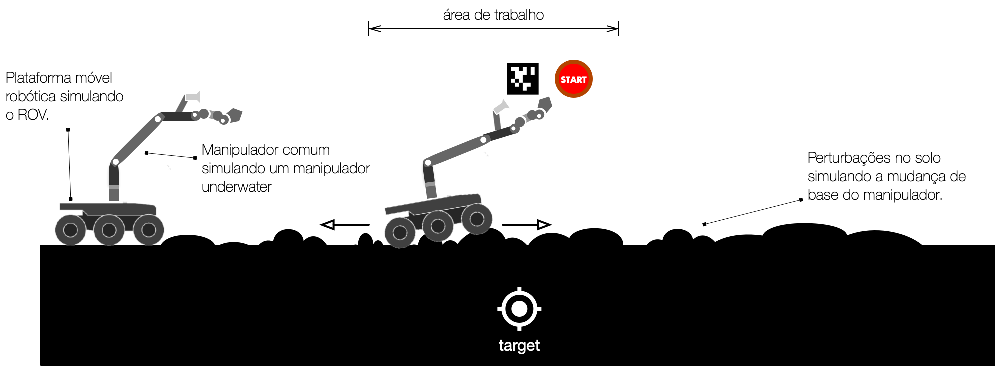
\includegraphics[width=1 \textwidth]{images/ManiSub_PoC.png} 
  \end{center} 
  \caption{Modelo representativo da prova de conceito.} 
  %\legend{Fonte: os autores.} 
  \label{fig:manipoc} 
\end{figure}
%\end{sidewaysfigure*}
%----------------------------

Para a demonstração da missão que o manipulador desenvolverá autonomamente, foi idealizado uma determinada região fixa para a plataforma móvel com um ponto referencial de fixação simulando o processo de ancoragem para o ROV, tendo estabelecido a ancoragem o sistema ficará sujeito às perturbações, que poderão ocorrer de forma aleatório ou não, dependendo somente da programação inicial que será levada em consideração na realização dos testes.

A próxima tarefa, o manipulador fará uma busca de reconhecimento com o intuito de encontrar um determinado marcador (Figura \ref{fig:apriltag}), que será capaz de informar ao manipulador para qual ponto da trajetória o mesmo deverá ir. Com a informação do ponto determinada, o sistema do manipulador deverá realizar cálculos de controle e de cinemática inversa em tempo real para a trajetória a ser desenvolvida. Este planejamento deverá, ao final do projeto, ser autônoma e precisa.

Com isso, o manipulador será capaz de realizar a missão para o qual foi planejado, que no caso deste projeto é o de apertar um botão, girar uma chave de emergência, inserir um pino no painel, realizar uma trajetória linear e uma circular, com o intuito de simular um processo de limpeza e uma inspeção em um \textit{pipeline} respectivamente.


%%%%%%% descrever a ideia

\subsection{Adaptação às condições operacionais}
\label{ssec:adap}
No desenvolvimento da prova de conceito é levada em consideração características operacionais que estejam em de acordo com a norma API RP 17H para o uso de ROVs de intervenção conforme Tabela xxx. Estas características são consideradas especificamente na simulação da prova de conceito. 




%
%%---- fase conceitual ------------------------------------
\subsection{Requisitos do cliente}
\label{ssec:reqcli-s}
A ideia apresentada na introdução desta seção tem como objetivo suprir com entendimento os requisitos levantados e impostos ao time de desenvolvimento quando do início do proejto.
Entendendo estas necessidades apontadas pelo cliente durante as reuniões realizadas, e analisando o plano de trabalho estabelecido, pode-se listar os seguintes requisitos primordiais para a realização deste projeto:
\begin{itemize}
	\item projetar, construir e demonstrar uma prova de conceito em laboratório para simular a automação de operações com ROVs que utilizam braços manipuladores;
	\item desenvolver um estudo de viabilidade técnico-econômica para automatizar algumas operações com ROVs, contendo os seguintes tópicos:
		\begin{itemize}
			\item Relação de operações usuais de ROVs e seus manipuladores;
			\item Estudo do estado da arte de ROVs;
			\item Estudo do estado da arte de manipuladores subaquáticos;
			\item Avaliação da complexidade das operações realizadas por ROVs e seus manipuladores;
			\item Avaliação do custo operacional dos manipuladores subaquáticos e o impacto nos custos totais das operações com ROVs;
			\item Estimação da redução de custos e tempos de operação quando da implementação da automação dos manipuladores;
			\item Estimação da redução dos riscos humanos principalmente referentes à prática de mergulho nas operações;
			\item Análise de risco da implementação da automação dos manipuladores;
			\item Avaliação da prontidão tecnológica para implementação da automação dos manipuladores;
			\item Análise de viabilidade técnico-econômica e impacto na operação da empresa.
		\end{itemize}
	\item elaborar um plano de trabalho, em decorrência da análise realizada no estudo de viabilidade, com o intuito de estabelecer um \textit{road map} para a aplicação de tecnologias apontadas no estudo.
\end{itemize}

Com três grandes entregáveis: prova de conceito, estudo de viabilidadse, e o plano de trabalho para o protótipo; o projeto estabelecerá respostas para cada requisito apresentado. O estudo de viabilidade foi iniciado com o levantamento dos requisitos e com a elaboração de questões a serem indagadas à equipe da PETROBRAS e aos fornecedores de equipamentos. Estas questões são apresentadas de forma preliminar no Apêndice \ref{ape:quest}, porém vale ressaltar que melhorias serão apontadas quando da realização do workshop no CENPES e no campo operacional de Macaé - RJ.

\section{Testes iniciais da simulação}
\label{sec:tstsim}
Para a prova de conceito que validará o controle de posição e trajetória de um manipulador submetido a perturbações 3D; uma forma de acelerar o desenvolvimento e focar nas funcionalidades requeridas para o manipulador é usar uma plataforma móvel que já esteja integrada com um manipulador. Além disso se o conjunto possuir câmera e unidade de processamento que possa processar algoritmos de mapeamento de imagens será um diferencial grande para o desenvolvimento. No entanto antes disso tudo, é necessário simular estes processos antes mesmo de submerter a implementação física.

Neste início de desenvolvimento, os compoonentes selecionados foram a plataforma robótica móvel do fabricante Clearpath  (Figura \ref{fig:jackal}) e o manipulador do fabricante Kinova (Figura \ref{fig:jaco2}).
%------ picture -------------
%\begin{sidewaysfigure*}
\begin{figure}[H] 
  \begin{center} 
  	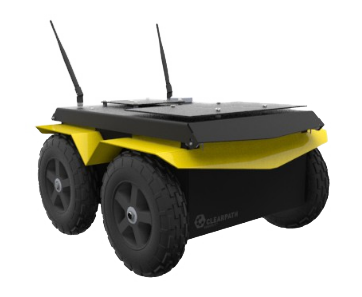
\includegraphics[width=0.5 \textwidth]{images/jackal.png} 
  \end{center} 
  \caption{Plataforma robótica móvel - Jackal.} 
  %\legend{Fonte: os autores.} 
  \label{fig:jackal} 
\end{figure}
%\end{sidewaysfigure*}
%----------------------------

%------ picture -------------
%\begin{sidewaysfigure*}
\begin{figure}[H] 
  \begin{center} 
  	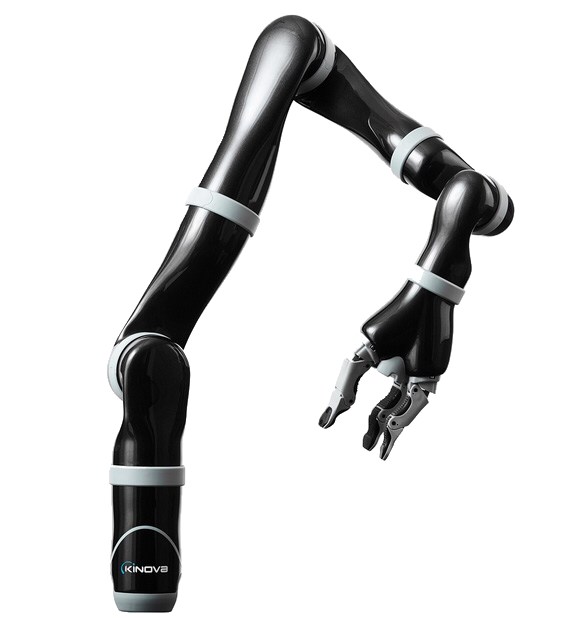
\includegraphics[width=0.4 \textwidth]{images/jaco2.png} 
  \end{center} 
  \caption{Manipulador - Jaco 2.} 
  %\legend{Fonte: os autores.} 
  \label{fig:jaco2} 
\end{figure}
%\end{sidewaysfigure*}
%----------------------------

Diante das informações obtidas dos fabricantes foi possível parametrizar as variáveis necessárias para que a simulação fosse a mais próxima do real. De forma a testar a idea principal no uso de manipuladores quando os mesmos são submetidos a perturbações e que a sua base é alterada aleatoriamente foi pensado em elaborar uma simulação utilizando o Pybullet \cite{pybullet} , que é uma plataforma em tempo real que simula as propriedade físicas de materiais de mecanismos robóticos.

O foco principal do teste foi elaborar uma trajetória pré-programada do manipulador e que durante o processo de trajetória sofresse uma perturbação em sua base.

O resultado esperado era o desempenho da trajetória na realização da missão, mostrando se eficaz na primeira tentativa, que era o de simplesmente permanecer no ponto esperado (Figura \ref{fig:jjsim}).
%------ picture -------------
%\begin{sidewaysfigure*}
\begin{figure}[H] 
  \begin{center} 
  	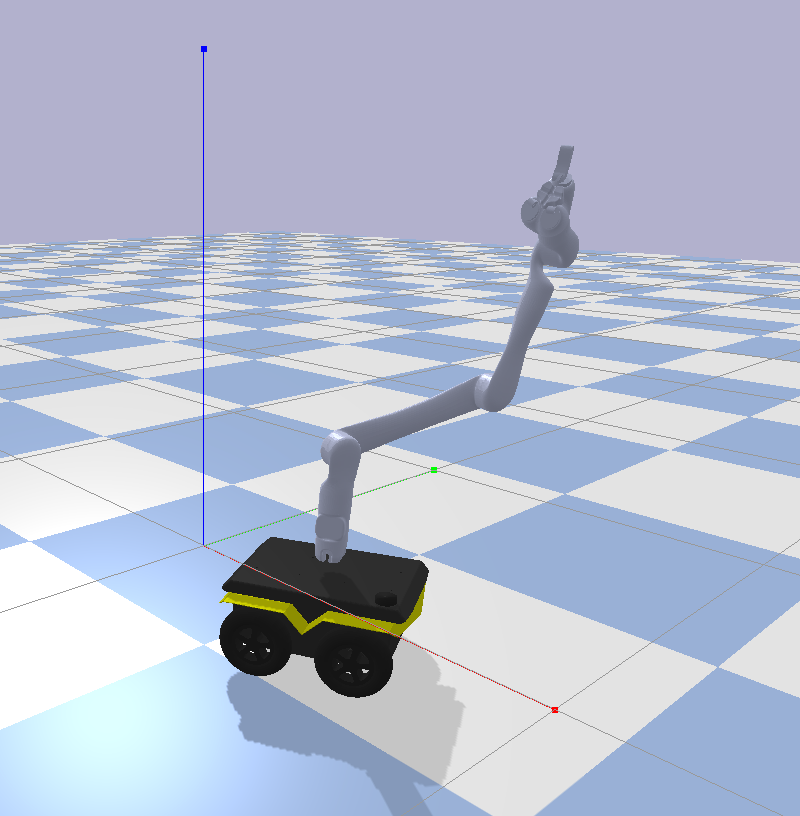
\includegraphics[width=0.4 \textwidth]{images/jjsim.png} 
  \end{center} 
  \caption{Modelo do sistema para a simulação.} 
  %\legend{Fonte: os autores.} 
  \label{fig:jjsim} 
\end{figure}
%\end{sidewaysfigure*}
%----------------------------

Com o resultado alcançado com o primeiro teste, em que o \textit{end-effector} tende a permanecer no ponto designado inicialmente, foi elaborado o segundo teste no qual requereria do \textit{end-effector} uma determinada tarefa a ser realizada mesmo tendo a base do manipulador alterada aleatoriamente.

Neste segundo teste, que está sendo apresentado na Figura \ref{fig:jjsimula} tem a intenção de apresentar uma certa sequência dos eventos realizados durante a simulação.
A tarefa desempenhada pelo \textit{end-effector} do manipulador foi o de descrever uma trajetória circular num determinado ponto.
Na Figura \ref{fig:jjsim1-1} o manipulador está na posição inicial da trajetória estipulada na missão, como consequência do evento o manipulador deve realizar uma trajetória que descreve uma circunferência no espaço (Figura \ref{fig:jjsim1-2}). Consequentemente após receber uma determinada perturbação de mudança na base do manipulador, o \textit{end-effector} permanece realizando a trajetória circular, conforme apresentado na Figura \ref{fig:jjsim1-3}.

O resultado do teste mostrou-se compatível com a ideia inicial em permanecer desenvolvendo a trajetória mesmo tendo a sua base fixa sofrendo perturbações em seus eixos.

\begin{figure}[ht]
	\begin{minipage}[t]{0.3\linewidth}
		%		\centering
		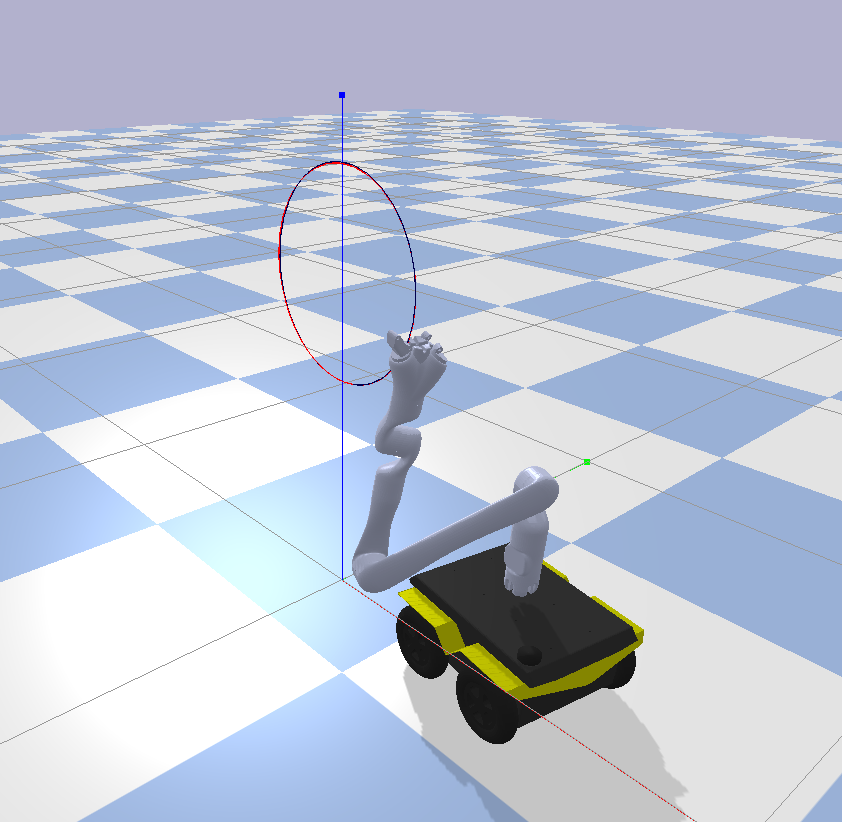
\includegraphics[width=1\textwidth]{images/jjsim1-1.png}
		\subcaption{Ponto inicial.}
		\label{fig:jjsim1-1}
	\end{minipage}
	\hfill
	\begin{minipage}[t]{0.3\linewidth}
		%		\centering
		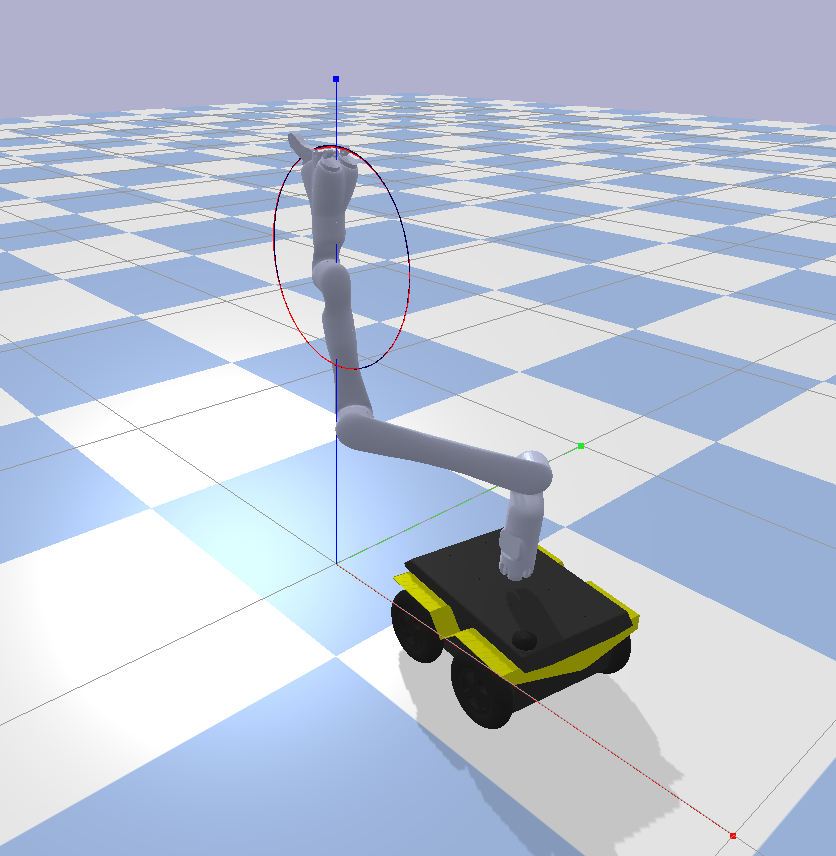
\includegraphics[width=1\textwidth]{images/jjsim1-2.png}
		\subcaption{Percorrendo um círculo.}
		\label{fig:jjsim1-2}
	\end{minipage}
	\hfill
	\begin{minipage}[t]{0.3\linewidth}
		%		\centering
		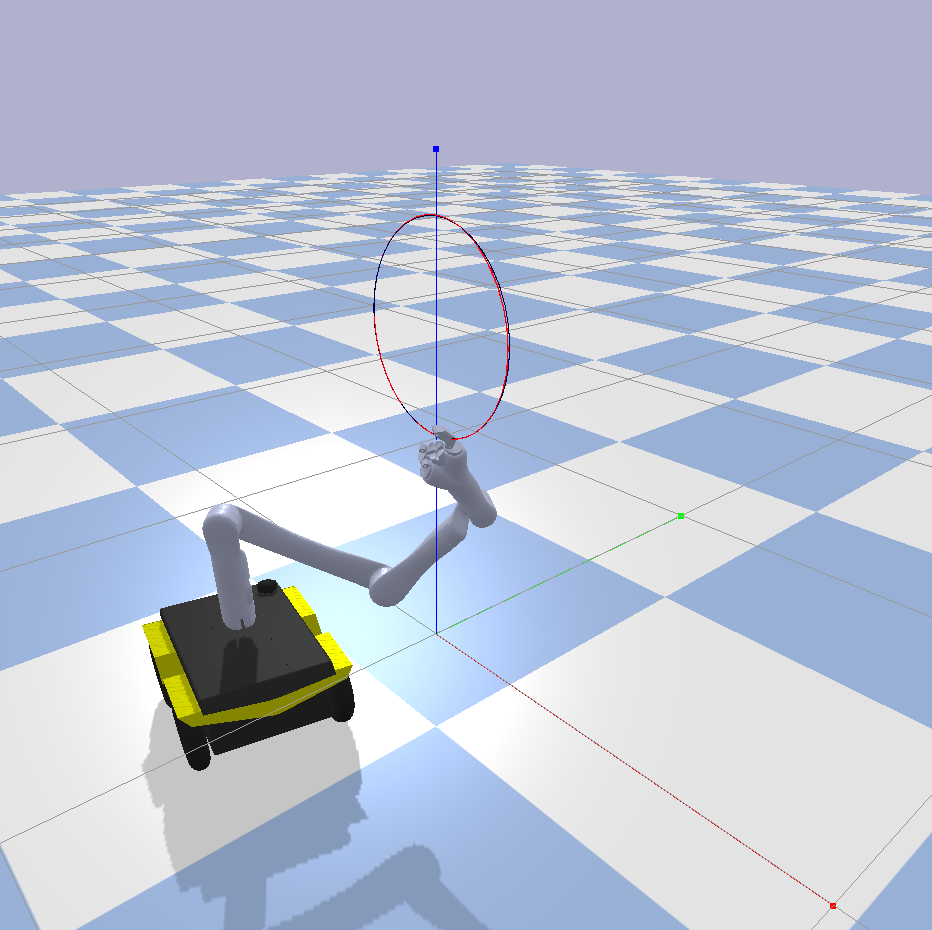
\includegraphics[width=1\textwidth]{images/jjsim1-3.png}
		\subcaption{Sistema com a base em um outra posição.}
		\label{fig:jjsim1-3}
	\end{minipage}  
	\caption{Simulação do sistema utilizando o PyBullet.}
	%\legend{Fonte: Própria.}
	\label{fig:jjsimula}
\end{figure}


%%---- fase conceitual ------------------------------------
%\section{Estudo do estado da arte}
%\label{sec:sota}
%
%
%
%%%---- fase conceitual ------------------------------------
%%\subsection{Benchmarking}
%%\label{sec:bnchmkg}
%
%%---- fase conceitual ------------------------------------
%\subsection{Ambiente de operação}
%\label{ssec:ambopt-s}

%%---- fase conceitual ------------------------------------
%\subsection{Normas aplicadas}
%\label{ssec:normas-s}


%\section{Análise técnica}
%\label{sec:an-tec-s}
%
%\subsection{Análise da avaliação da prontidão tecnológica}
%\label{sec:an-trl-s}
%
%
%\section{Análise econômica}
%\label{sec:an-eco-s}
%
%\subsection{Análise de risco}
%\label{sec:an-rsk-s}
%




	%%=========================================================
%---- fase conceitual ------------------------------------
%=========================================================
%\chapter{BASIS OF DESIGN}
%\label{chap:bod}
%
%%---- fase conceitual ------------------------------------
%\section{Requisitos do cliente}
%\label{sec:reqcli}
%
%%---- fase conceitual ------------------------------------
%\section{Estudo do estado da arte}
%\label{sec:sota}
%
%%---- fase conceitual ------------------------------------
%\subsection{Benchmarking}
%\label{sec:bnchmkg}
%
%%---- fase conceitual ------------------------------------
%\section{Ambiente de operação}
%\label{sec:ambopt}
%
%%---- fase conceitual ------------------------------------
%\section{Normas}
%\label{sec:normas}


\chapter{ANÁLISE DE VIABILIDADE}
\label{chap:an-via}


\section{Viabilidade técnica}
\label{sec:via-tec}


\section{Viabilidade financeira}
\label{sec:via-fin}







	%=========================================================
%---- fase conceitual ------------------------------------
%=========================================================
\chapter{CONCEITO DO SISTEMA}
\label{chap:sist}

%---- fase conceitual ------------------------------------
\section{Arquitetura geral}
\label{sec:arqger}

%---- fase conceitual ------------------------------------
\section{Estrutura analítica do protótipo}
\label{sec:eap}

%---- fase conceitual ------------------------------------
\section{Especificação técnica do sistema}
\label{sec:esptec}

%---- fase conceitual ------------------------------------
\subsection{Matrix morfológica}
\label{sec:mtxmorf}

%---- fase conceitual ------------------------------------
\subsection{Componentes principais}
\label{sec:compprinc}

%---- fase conceitual ------------------------------------
\subsection{Desdobramento da função Qualidade}
\label{sec:qfd}

%---- fase conceitual ------------------------------------
\subsubsection{Requisitos do cliente e técnicos}
\label{sec:reqclitec}

%---- fase design ----------------------------------------
\subsubsection{Requisitos técnicos e funcionalidades}
\label{sec:reqtecfunc}



	%---- fase design ----------------------------------------%
%
% \chapter{ESPECIFICAÇÃO FUNCIONAL}
% \label{chap:espfunc}

% %---- fase design ----------------------------------------
% \section{Funcionalidade}
% \label{sec:func1}

% %---- fase design ----------------------------------------
% \subsection{Descrição}
% \label{sec:desc1}

% %---- fase design ----------------------------------------
% \subsection{Premissas necessárias}
% \label{sec:prem1}

% %---- fase design ----------------------------------------
% \subsection{Dependências}
% \label{sec:dep1}

% %---- fase design ----------------------------------------
% \subsection{Saídas}
% \label{sec:said1}


\chapter{ANÁLISE ECONÔMICAx}
\label{chap:rsk}

%---- Análise de custos das operações com ROV ------------------------------------
\section{Análise de custos}
\label{sec:rskconc}
Os custos com operações offshore receberam limitada atenção dos meios acadêmico e corporativo. Em boa parte, os custos com a produção com petróleo e gás ocupam uma pequena porção orçamentária, além dos altos preços das commodities gerarem grandes fluxos de caixa, aumentando a produção e vendas por consequência (KAISER, 2019).

Diferente dos custos de capital para prospecção de petróleo e seus derivados, os custos operacionais são menos transparentes , com menor disponibilidade de dados e informações pertinentes para avaliação, vindo de diferentes formas e aplicações. Apesar de tais obstáculos, há estudos de benchmark que propuseram diminuir o gap entre as informações obtidas e a avaliação resultante do processo, obtendo relativo êxito em suas execuções. 

A proposta desta seção é avaliar os custos associados ao uso de manipuladores subaquáticos em ROVs. Para isso, os dados foram coletados e utilizados segundo informações da Petrobras a cerca dos contratos de embarcação de ROV para inspeção, reparo e manutenção, conforme apresentado na Tabela \ref{tab:cost1}:

\begin{table}[h!]
    \centering
	\begin{threeparttable}
	\centering
	\caption{Variáveis de embarcação tipo RSV}
	\label{tab:cost1}
    \begin{tabular}{p{8cm} >{\centering\arraybackslash}m{3.7cm}}
    %\begin{tabular}{l c}
		\hline
		\multicolumn{1}{c}{\textbf{Variáveis}} & \textbf{Valores}\tnote{i}  \\ \hline
		Diária RSV                              & US\$81.474,45     \\
		Ciclo 28 dias                          & US\$2.281.284,60  \\
		Total contrato RSV                     & US\$44.667.552,47 \\
		Total dias de contrato                 & 547               \\
		&                   \\
		Total de operações (A)\tnote{ii}                 & 1976              \\
		Total de inspeções                     & 1337              \\
		Total de intervenções                  & 639               \\
		Número de anomalias (B)                & 432               \\
		Índice de anomalias (B/A)              & 21,86\%           \\ \hline
	\end{tabular}
\begin{tablenotes}
\item[i]{Valores monetários a US\$ correntes}
\item[ii]{Operações e anomalias tiveram seus valores projetados para um ciclo contratual de 547 dias.}
\end{tablenotes}
\end{threeparttable}
\end{table}


Pode-se observar que os contratos de embarcação tipo RSV (ROV Support Vessel) da Petrobras são realizados em ciclos de 28 dias\footnote{Há também outros contratos internacionais que estabelecem um dia útil de 12 horas de trabalho, com permissão máxima de inatividade do ROV de 30 horas por mês (KAISER, 2019).} , com 1 dia de manutenção e reparo de equipamentos, alcançando a diária aproximada de US\$ 81 mil\footnote{Alguns estudos empíricos registram taxas diárias para RSV entre 100 e 300 mil dólares, dependendo do tamanho da embarcação utilizada.}. O valor da diária inclui, além do afretamento, materiais, equipamentos, bens importados e tripulação. 

Para gerar efeitos comparativos mais precisos, e considerando o uso da embarcação por 24 horas, as atividades descritas nos conjuntos da Tabela 1 terão o valor da diária estabelecido em minutos. A ideia consiste em mensurar a participação de uma determinada atividade em relação ao total previsto em um dia completo de operações. 
Estabeleceu-se a divisão das operações por conjunto segundo o nível de complexidade inerente à sua realização, i.é., o Conjunto 1 pode demandar um tempo menor de execução se comparado aos Conjuntos 3 e 4, por exemplo. As médias apresentadas na tabela seguem a seguinte estrutura:

\begin{table}[h!]
    \centering
    \resizebox{\textwidth}{!}{
	\begin{threeparttable}
	\centering
	\caption{Variáveis de embarcação tipo RSV}
	\label{tab:cost1}
    \begin{tabular}{l >{\centering\arraybackslash}m{3.0cm} >{\centering\arraybackslash}m{3.0cm} >{\centering\arraybackslash}m{3.0cm}}
		\hline
        \textbf{Operação submarina\tnote{i}}           & \textbf{Frequência média mensal} & {\textbf{Sem automação (min)}} & \textbf{Com automação (min)} \\ \hline
		Conjunto 1                                     &                                  &                                &                              \\
		\hspace{3mm}Abertura e fechamento de válvulas  & 12                               & 10                             & 5                            \\
		\hspace{3mm}Colocação e retirada de hot stab   & 28                               & 10                             & 4                            \\
		\hspace{3mm}Uso de torque tool                 & 12                               & 15                             & 5                            \\
		Conjunto 2                                     &                                  &                                &                              \\
		\hspace{3mm}Instalação de \textit{tree cap}    & 5                                & 60                             & 30                           \\
		\hspace{3mm}Conexão de \textit{flying leads}   & 10                               & 60                             & 15                           \\
		Conjunto 3                                     &                                  &                                &                              \\
		\hspace{3mm}Limpeza de \textit{hub}\tnote{ii}  & 5                                & 240                            & 60                           \\
		Conjunto 4                                     &                                  &                                &                              \\
		\hspace{3mm}Instalação de flanges              & 5                                & 180                            & 60                           \\ \hline
	\end{tabular}
    \begin{tablenotes}
        \item[i]{Valores monetários a US\$ correntes}
        \item[ii]{Operações e anomalias tiveram seus valores projetados para um ciclo contratual de 547 dias.}
    \end{tablenotes}
    \end{threeparttable}
    }
\end{table}

A hipótese central para os valores presentes no item C está em aproximar mais precisamente os tempos de execução das atividades presentes nos registros dos melhores condutores dos manipuladores. Por mais que estes tenham a experiência para uma boa condução, ainda há fatores (sejam eles de caráter endógeno ou exógeno) que possibilitam a presença de anomalias, enquanto com a automação estas seriam minimizadas.

O conjunto 1 corresponde às atividades que envolvem acionamento mecânico de válvulas submarinas com o ROV equipado com ferramentas de torque (\textit{torque tool}). Tal conjunto relaciona-se com os demais porque estes dependem diretamente do acionamento de válvulas para que ocorra a instalação/desinstalação de determinados equipamentos, o que justifica a maior frequência de manuseios de válvulas e \textit{torque tools}. Apesar de a Petrobras estabelecer máximo de 15 minutos para movimentos envolvendo válvulas, há registros apontando para valores médios de 10 minutos, com aproximação da média com automação em 5 minutos, uma diminuição de aproximadamente 50\% em relação à média máxima esperada em contrato.

O lançamento/instalação de \textit{Tree Cap} em árvore de natal molhada (ANM) e manuseio de \textit{flying leads}, utilizando ferramenta de torque, compõem o conjunto 2 de serviços do ROV. O principal diferencial para diminuição do tempo de execução em \textit{flying leads} está na presença de uma ferramenta de orientação inserida (FLOT) no ROV para colocá-los na ANM, que pode chegar em até 1/3 do valor comparado ao FLOT não residente. Para fins didáticos, o estudo propôs trabalhar somente com os valores onde há a utilização da ferramenta de orientação, registrando um total de execução de 60 minutos entre instalação e desinstalação dos componentes.

A operação de limpeza de \textit{hubs}, atividade fundamental do Conjunto 3, consiste em remover incrustações e/ou vidas marinhas dos equipamentos a partir de ferramentas de limpeza operadas por ROVs a fim de permitir instalação de subequipamentos. Em certas ocasiões, a limpeza do \textit{hub} está associada à necessidade de retirar as capas de proteção ou capas de teste. Por este motivo, quando realizadas no mesmo período programado, desinstalações de \textit{tree caps} (Conjunto 2) podem interferir diretamente no tempo de execução da limpeza do \textit{hub}, apresentando a maior média de tempo dentre todos os conjuntos de atividades no estudo. Ademais, a atividade em si depende muito da experiência do condutor do ROV e, dentro dos relatos da Petrobras, possui as maiores probabilidades de apresentar anomalias, gerando maiores desvios padrões em relação à média observada. Os valores representados na Tabela 1 para tal conjunto são equivalentes ao tempo médio de somente a realização da limpeza (4 horas aproximadamente).  

Por fim, o Conjunto 4 consiste na instalação de flanges cego (ou cubo cego \textit{grayloc}\footnote{Tecnologia desenvolvida por Oceaneering. Para mais informações, ver: https://www.oceaneering.com/grayloc-technology (acesso em 29/10/2019).}) em conexões de dutos rígidos e flexíveis, a partir de materiais fornecidos pela Petrobras. O conjunto envolve preparação e manuseio do flange no convés, lançamento, instalação de estojos, torqueamento e teste de estaqueidade. Dentro das atividades previstas, a instalação de estojos é a que possui maior interdependência entre os outros conjuntos de atividades descritas anteriormente, envolvendo inspeção visual, limpeza, destorqueamento, medição de potencial eletroquímico, instalação e torqueamento do novo estojo. Desta forma, torna-se mais complexa\footnote{Parte dessa complexidade também diz respeito ao uso correto da ferramenta, que deve possuir \textit{handles} em múltiplas posições para facilitar o manuseio pelo manipulador do ROV.}  a mensuração da performance. Para este estudo, a média de tempo para execução adotada foi de 180 minutos, podendo apresentar o mesmo comportamento observado no Conjunto 3.  

Dada a apresentação da estrutura dos conjuntos de atividades com manipuladores de ROV, deu-se prosseguimento à conversão dos dados em unidades monetárias para mensurar as proporções desses custos em relação à diária da embarcação, considerando para o caso somente as operações de intervenção\footnote{Apesar de haver uso de manipuladores para inspeções para casos de limpeza e medição de potencial eletroquímico, sua mensuração em tempo de execução é mais assertiva em inspeções programadas.}. Essa elaboração pode ser observada na Tabela 2, com os valores aproximados por minuto de uma diária completa de atividades, isto é, 24 horas (ou 1440 minutos) ininterruptas de prestação de serviço. 

\begin{table}[h!]
	\centering
	\caption{Dados monetários dos conjuntos de atividades em ROV}
	\label{tab:cost3}
	\def\arraystretch{1.2}
	\resizebox{\textwidth}{!}{%
		\begin{tabular}{llccc}
			\hline
            \multicolumn{2}{c}{\textbf{Operação submarina}} & \textbf{\begin{tabular}[c]{@{}c@{}}Valor médio de execução (US\$) \\ (A)\end{tabular}} & \textbf{\begin{tabular}[c]{@{}c@{}}Valor esperado com automação \\ (B)\end{tabular}} & \textbf{\begin{tabular}[c]{@{}c@{}}$\Delta$ A/B \\ (\%)\end{tabular}} \\ \hline
			\multicolumn{2}{l}{Conjunto 1}                  & \multicolumn{1}{l}{}                                                                   & \multicolumn{1}{l}{}                                                                 & \multicolumn{1}{l}{}                                          \\
			& Abertura e fechamento de válvulas      & 6.789,54                                                                               & 3.394,77                                                                             & 50\%                                                          \\
			& Colocação e retirada de hot stab       & 15.842,25                                                                              & 6.336,90                                                                             & 60\%                                                          \\
			& Uso de torque tool                     & 10.184,31                                                                              & 3.394,77                                                                             & 67\%                                                          \\
			\multicolumn{2}{l}{Conjunto 2}                  &                                                                                        &                                                                                      &                                                               \\
			& Instalação de tree cap                 & 16.973,84                                                                              & 8.486,92                                                                             & 50\%                                                          \\
			& Conexão de flying leads                & 33.947,69                                                                              & 8.486,92                                                                             & 75\%                                                          \\
			\multicolumn{2}{l}{Conjunto 3}                  &                                                                                        &                                                                                      &                                                               \\
			& Limpeza de hub                         & 67.895,38                                                                              & 16.973,84                                                                            & 75\%                                                          \\
			\multicolumn{2}{l}{Conjunto 4}                  &                                                                                        &                                                                                      &                                                               \\
			& Instalação de flanges                  & 50.921,53                                                                              & 16.973,84                                                                            & 67\%                                                          \\ \hline
		\end{tabular}%
	}
\end{table}
Observando os dados oriundos da Tabela 2, nota-se que as argumentações anteriormente apresentadas corroboram com os valores monetários expressos, sobretudo na interdependência dos Conjuntos 3 e 4 em relação às atividades mais ordinárias. É evidente que os dados apresentem proporções diretas com o presente na Tabela 1, visto que foram multiplicados por um valor constante (valor da diária de embarcação por minuto), o que justifica as variações percentuais entre 50 e 75\% das médias sem e com intermédio da automação, respectivamente.

Ademais, pode-se esperar margens ainda maiores com as atividades que possuem tempos de execução com alto desvio-padrão, como é o caso da instalação de \textit{tree cap} e da limpeza de \textit{hub}. 

Ao realizar a soma dos valores monetários dos conjuntos, obtêm-se algumas importantes observações e desdobramentos, que podem ser verificados na Tabela 3.

\begin{table}[h!]
	\centering
	\caption{Soma dos custos das atividades com manipuladores}
	\label{tab:cost4}
	\def\arraystretch{1.2}
	\resizebox{\textwidth}{!}{%
		\begin{tabular}{llll}
			\hline
			\textbf{Conjunto de Operações} & \textbf{Valor sem automação (A)} & \textbf{Valor com automação (B)} & \textbf{Redução (A - B)} \\ \hline
			Conjunto 1                     & 32.816,10                        & 13.126,44                        & 19.689,66                \\
			Conjunto 2                     & 50.921,53                        & 16.973,84                        & 33.947,69                \\
			Conjunto 3                     & 67.895,38                        & 16.973,84                        & 50.921,53                \\
			Conjunto 4                     & 50.921,53                        & 16.973,84                        & 33.947,69                \\
			\textbf{Total}                 & \textbf{202.554,54}              & \textbf{64.047,97}               & \textbf{138.506,57}      \\ \hline
		\end{tabular}%
	}
\end{table}

Com os valores monetários expressos na Tabela 3, espera-se que haja uma redução de custos de aproximadamente 59\%  \footnote{O percentual não englobou os custos associados a pessoal e logística, assim como a depreciação, reparos e manutenções necessárias.}em relação aos conjuntos de operações realizados sem automação. Visto que são valores representativos a duas instalações simultâneas em árvores de natal molhada por mês, esses podem obter um impacto ainda mais significativo se analisado em período anual.

Além dos impactos diretos nos custos com as operações dos manipuladores, outros possíveis efeitos indiretos devem ser considerados como, por exemplo, a minimização de anomalias em riscos ambientais e diminuição do consumo de óleo diesel, necessário para o funcionamento das embarcações de ROVs. 

Por fim, vale destacar a importância de um conjunto de atividades específicas ao monitoramento sísmico marítimo utilizando receptores pontuais (também conhecidos como \textit{nodes}). 

Por ser uma tecnologia disruptiva, pioneira no âmbito mundial, ela servirá para gerenciamento da produção dos reservatórios do Pré-Sal da Bacia de Santos. As hipóteses para sua implementação são os ganhos de qualidade intrínseca dos dados sísmicos - incluindo qualidade sísmica 4D - e ganhos de tempo de processamento destes dados. Além da maior flexibilidade operacional e qualidade dos dados, o conceito terá uma rápida capacidade de apropriação pela Petrobras, uma vez que a tecnologia já está madura e amplamente desenvolvida na empresa\footnote{Um exemplo desse domínio são as estacas-torpedos, empregadas como meio de baixo custo para enterramento dos \textit{nodes}.}.

As etapas previstas para as quais a tecnologia deverá passar são: 

\begin{itemize}
	\item Prototipagem, que inclui a produção de uma maquete em escala reduzida;
	\item Validação dos componentes e do sistema em escala laboratorial, ainda na fase de P\&D;
	\item Testes em escala reduzida, ambiente controlado e incluindo a estaca instrumentada;
	\item Produção de cinco unidades constituídas de um Módulo Submarino de Aquisição de Dados Sísmicos (MSADS) e um Dispositivo de Transporte e Liberação de Estacas (DLTE);
	\item Teste de campo para validação da operação em condições realistas;
	\item Avaliação da prova de conceito final e recomendações para manufatura em escala comercial.
\end{itemize}

A justificativa para tal conceito estar dentro do estudo encontra-se nas operações do ROV com o Módulo de Estaca-Suporte (MES), MSADS, Módulo de Posicionamento e Alinhamento (MPA), sendo estas necessárias tanto para operações de instalação quanto de desinstalação dos componentes, cujos tempos de execução sem a automação e os previstos com a implementação da automação dos manipuladores podem ser observados na Tabela 4.

\begin{table}[h!]
	\centering
	\caption{Tempos de execução com operações do MSADS}
	\label{tab:node1}
	\def\arraystretch{1.2}
	\resizebox{\textwidth}{!}{%
		\begin{tabular}{llcc}
			\hline
			& \textbf{}                                                          & \multicolumn{2}{c}{\textbf{Duração}}                                                                                                    \\ \hline
			& \multicolumn{1}{c}{\textbf{Etapa/Descrição}}                       & \textbf{\begin{tabular}[c]{@{}c@{}}Manual \\ (min)\end{tabular}} & \textbf{\begin{tabular}[c]{@{}c@{}}Automático \\ (min)\end{tabular}} \\ \hline
			\multicolumn{2}{l}{Instalação}                                        & \multicolumn{1}{l}{}                                             & \multicolumn{1}{l}{}                                                 \\
			& Posicionar o MSADS no disco da estaca                              & 12                                                               & 5                                                                    \\
			& Retirar capa protetora do conector elétrico e colocá-la no suporte & 14                                                               & 6                                                                    \\
			& Retirar conector elétrico no jumper e colocar em painel de estaca  & 15                                                               & 6                                                                    \\
			\multicolumn{2}{l}{Desinstalação}                                     &                                                                  &                                                                      \\
			& Desconectar do jumper do painel e colocar o conector elétrico      & 12                                                               & 5                                                                    \\
			& Recolocar a capa protetora no painel de estaca                     & 14                                                               & 6                                                                    \\
			& Retirar o MSADS do disco da estaca                                 & 11                                                               & 4                                                                    \\ \hline
		\end{tabular}%
	}
\end{table}

As etapas das operações que necessitam do auxílio do ROV consistem em lançar várias estacas-suporte em ambiente submarino, conectar os módulos permanentes e não-permanentes, registro sísmico, desconexão do módulo de eletrônica e recuperação dos dados registrados.  

O MSADS, também conhecido como Módulo de Eletrônica, contém um suporte para que este seja suspenso por um ROV, além de um conector de conexão molhada, manuseável pelo manipulador presente no veículo, para colocá-lo ao painel da Estaca-suporte. 

Inicialmente posiciona-se o MSADS no disco de estaca, procedimento que leva em média 12 minutos para execução. Em seguida, retira-se a capa protetora do conector elétrico no painel da estaca e coloca essa em seu suporte no painel, com uma estimativa de execução de aproximadamente 14 minutos. Compondo a etapa final de instalação, há a retirada do conector elétrico na extremidade do \textit{jumper}\footnote{Operações de conexões e desconexões de \textit{jumper} elétrico consistem em realizar interligações/desconexões elétrica entre equipamentos e/ou subequipamentos submarinos com a finalidade de permitir comando e monitoramento eletroeletrônico a partir da superfície.}  no MSADS e realiza-se a conexão deste no painel da estaca, com tempo estimado de 15 minutos para realização. Espera-se que, com a automação dos manipuladores, haja uma redução média de 24 minutos entre todas as operações de instalação.

Para os processos de desinstalação, de início, a primeira etapa consiste em desconectar o \textit{jumper} do painel da estaca e colocar o conector elétrico do \textit{jumper} em seu suporte no Módulo de Eletrônica, com duração aproximada de 12 minutos. A etapa seguinte procura recolocar a capa protetora no conector elétrico do painel da Estaca-suporte, levando em média 14 minutos para sua execução. Por fim, realiza-se a operação de retirada do MSADS do disco de estaca por volta de 11 minutos. Da mesma maneira que nas instalações, com a automação espera-se que haja uma redução total cerca de 22 minutos.

\begin{table}[h!]
	\centering
	\caption{Valores das atividades realizadas com nodes}
	\label{tab:node2}
	\def\arraystretch{1.2}
	\resizebox{\textwidth}{!}{%
		\begin{tabular}{llccc}
			\hline
			&                                                       & \multicolumn{3}{c}{\textbf{Valores (diária)}}                                                                                                                                                                   \\ \hline
			& \multicolumn{1}{c}{\textbf{Etapa/Descrição}}          & \textbf{\begin{tabular}[c]{@{}c@{}}Manual (US\$) \\ (A)\end{tabular}} & \textbf{\begin{tabular}[c]{@{}c@{}}Automático (US\$)\\ (B)\end{tabular}} & \textbf{\begin{tabular}[c]{@{}c@{}}A/B \\ (\%)\end{tabular}} \\ \hline
			\multicolumn{2}{l}{Instalação}                           & \multicolumn{1}{l}{}                                                  & \multicolumn{1}{l}{}                                                     & \multicolumn{1}{l}{}                                         \\
			& Posicionamento do MSADS no disco da estaca            & 1.250,00                                                              & 520,83                                                                   & 58,33                                                        \\
			& Retirar e colocar capa protetora do conector elétrico & 1.458,33                                                              & 625,00                                                                   & 57,14                                                        \\
			& Retirar e colocar conector elétrico no jumper         & 1.562,50                                                              & 625,00                                                                   & 60,00                                                        \\
			\multicolumn{2}{l}{Desinstalação}                        &                                                                       &                                                                          &                                                              \\
			& Desconectar do jumper e colocar o conector elétrico   & 1.250,00                                                              & 520,83                                                                   & 58,33                                                        \\
			& Recolocar a capa protetora no conector elétrico       & 1.458,33                                                              & 625,00                                                                   & 57,14                                                        \\
			& Retirar o MSADS do disco da estaca                    & 1.145,83                                                              & 416,67                                                                   & 63,64                                                        \\ \hline
		\end{tabular}%
	}
\end{table}
De maneira análoga ao apresentado nas Tabelas 2 e 3, os dados dos tempos de execução em operações com os módulos submarinos foram multiplicados por um valor da diária de embarcação proporcional por minuto. Para operações como essas, a embarcação mais adequada é a de pesquisa sísmica, cujo valor adotado foi de US\$161,9 mil\footnote{Tanto em relatórios anuais das empresas prestadoras de serviços quanto a literatura acadêmica empírica utilizam de uma margem que, para os valores correntes, chegam entre US\$150 e US\$200 mil.} , e que pode ser observado na Tabela 5. 

As variações percentuais presentes na última coluna corroboram a importância da automação nos processos envolvendo monitoramento sísmico\footnote{Vale ressaltar que a instalação do Módulo de Posicionamento e Alinhamento (MPA) também pode ser autônomas. Para tal, espera-se que haja uma redução de 2 minutos, em média, entre as operações sem e com automação. Por ser uma oportunidade tecnológica em fase de exploração pela Petrobras, não há dados monetários concretos para serem levantados.}. Por   permanente. Os valores monetários expressos podem ainda sofrer alterações significativas dependendo da diária estabelecida em contrato, dentro dos padrões internacionais para este tipo de atividade. Quando representados em um período contratual de uma embarcação de pesquisa sísmica, as operações elucidadas na Tabela 5 possuem amplas margens de redução de custo com a automação.

\begin{table}[h!]
	\centering
	\caption{Valores proporcionais em período de contratação - nodes}
	\label{tab:node3}
	\def\arraystretch{1.2}
	\resizebox{\textwidth}{!}{%
		\begin{tabular}{lllll}
			\hline
			\multicolumn{1}{c}{\textbf{Tipo de operação}} & \multicolumn{1}{c}{\textbf{\begin{tabular}[c]{@{}c@{}}Manual (US\$ 1000) \\ mín\end{tabular}}} & \multicolumn{1}{c}{\textbf{\begin{tabular}[c]{@{}c@{}}Automático (US\$ 1000) \\ mín\end{tabular}}} & \multicolumn{1}{c}{\textbf{\begin{tabular}[c]{@{}c@{}}Manual (US\$ 1000) \\ máx\end{tabular}}} & \multicolumn{1}{c}{\textbf{\begin{tabular}[c]{@{}c@{}}Automático (US\$ 1000) \\ máx\end{tabular}}} \\ \hline
			Instalação                                    & 4.609,47                                                                                       & 1.911,24                                                                                           & 27.656,81                                                                                      & 11.467,46                                                                                          \\
			Desinstalação                                 & 4.159,76                                                                                       & 1.686,39                                                                                           & 24.958,58                                                                                      & 10.118,34                                                                                          \\
			\textbf{Total}                                & \textbf{8.769,23}                                                                              & \textbf{3.597,63}                                                                                  & \textbf{52.615,39}                                                                             & \textbf{21.585,80}                                                                                 \\
			\textbf{Diferença}                            & \textbf{-}                                                                                     & \textbf{5.171,60}                                                                                  & \textbf{-}                                                                                     & \textbf{31.029,59}                                                                                 \\ \hline
		\end{tabular}%
	}
\end{table}

Quando agregadas as atividades de instalação e desinstalação dos Módulos de Eletrônica, a redução de custo pode variar de 5,2 a 31 milhões de dólares por contrato. A justificativa para o desvio padrão apresentado está na quantidade de intervenções já realizadas até então pela Petrobras por ciclos contratuais. Ademais, tal desvio padrão viabiliza as oportunidades tecnológicas presentes na automação do monitoramento sísmico, com o escopo de 2 anos e meio para tornar o sistema no mínimo semi-operacional.

Em suma, do ponto de vista financeiro, espera-se que a automação provenha reduções significativas de custos associadas aos manipuladores de ROV, seja em operações mais ordinárias, como aberturas e fechamentos de válvulas, seja em operações onde a Petrobras obterá o pioneirismo mundial, como nas operações de intervenções em \textit{nodes all-in-two}. 

Entretanto, para que a automação dos manipuladores seja considerada viável no âmbito econômico, verificou-se a necessidade de se avaliar a rentabilidade dos projetos de P\&D associados, em uma metodologia de valoração amplamente utilizada por empresas e academia, e que será explorada na seção seguinte. 


%---- Modelo de Valoração P&D ----------------------------------------
\section{Modelo de valoração dos projetos de P\&D}
\label{sec:rskdesig}

A fim de obterem vantagens competitivas que proporcionem lucros monopolísticos\footnote{A busca de oportunidades ou inovação, em seu sentido mais amplo, geram monopólios temporários, de menor ou maior período, até que sejam desafiados por novos concorrentes ou imitadores, tornando a concorrência um processo ativo e evolutivo de espaço e oportunidades tecnológicos. Para mais, ver Possas(2005).} , as empresas buscam inovações e o mercado, consequentemente, selecionam os resultados econômicos oriundos dessas mesmas inovações através de decisões estratégicas. 

Essas estratégias podem ocorrer através de investimentos em P\&D, atuando como ativos intangíveis e cujos esforços convertem-se em desenvolvimento de novos produtos, processos e/ou serviços. Os resultados deste processo são observáveis através dos impactos gerados na esfera empresarial, ou até mesmo no âmbito socioeconômico. 

No entanto, como discutido na introdução, os esforços para se investir em P\&D possuem incertezas inerentes que tornam a atividades de difícil avaliação ex-ante. Para isso, a Teoria de Opções Reais apresenta-se como um método robusto para análises de cenários onde há presença de incerteza e flexibilidade gerencial de longo prazo (DIXIT \& PYNDICK, 1994; MUN, 2002). 

Considerando que todo projeto de P\&D é, em essência, um projeto de investimento produtivo, este pode ser visto como um conjunto de opções reais. Dentre tais opções, as empresas detêm a capacidade de optar de adiar o investimento, cancelar novas etapas, alterar a escala produtiva (como é o caso de expansão e contração), abandonar por conta do excessivo ônus e opções de crescimento (MEIRELLES, 2004). 

Para a construção da análise, utilizaram-se dados provenientes da última demonstração financeira da Petrobras e dos esforços de P\&D, que estarão concentrados integralmente nos recursos alocados e esperados em parceria com o SENAI CIMATEC, e que podem ser observados na Tabela 6.

\begin{table}[h!]
	\centering
	\caption{Variáveis utilizadas para modelo de valoração}
	\label{tab:valor1}
	\def\arraystretch{1.2}
	\begin{tabular}{lc}
		\hline
		\multicolumn{1}{c}{\textbf{Variáveis}} & \textbf{Valor} \\ \hline
		Investimento na Fase 1                 & R\$ 1,34 mi    \\
		Investimento na Fase 2                 & R\$ 18 mi      \\
		VPL descontado                         & R\$ 20,23 mi   \\
		Volatilidade                           & 25\%           \\
		Taxa risk-free                         & 5\%            \\
		Período da Fase 1                      & 1 ano          \\
		Período da Fase 2                      & 2 anos         \\ \hline
	\end{tabular}
\end{table}

O investimento para o projeto foi dividido em duas grandes fases: inicialmente, o desenvolvimento viável das provas de conceito para, em seguida, testar o desempenho da automação dos manipuladores em ambientes reais. Para isso, estima-se investimentos de aproximadamente R\$ 19,34 milhões em um período de 3 anos. Utilizando a simulação Monte Carlo, e baseado na convergência das respostas dos pesquisadores com a metodologia A$Dˆ2$ (Advancement Degree of Difficulty)\footnote{A metodologia baseia-se na mensuração das dificuldades previstas no projeto para amadurecer o uso da tecnologia. Variáveis como custo, cronograma e os riscos inerentes às fases do projeto são consideradas na avaliação.} , a volatilidade implícita dos fluxos de caixa esperados com o projeto é de 25\%. 

Para a valoração estática dos lucros futuros, utilizou-se o modelo de fluxos de caixa descontado por uma taxa de desconto baseada no custo médio ponderado sobre o capital. A partir dos dados provenientes das demonstrações financeiras, a Petrobras teve, em 2018, 290 propriedades intelectuais (em grande parte, patentes) concedidas no Brasil e exterior. O valor adicionado recebido em alugueis, royalties e outros por conta de tais propriedades ficou em torno de R\$1,1 bilhão. Constatando os valores adicionados em períodos anteriores e dividindo pelas patentes concedidas, calculou-se o valor de R\$2,62 milhões por concessão, que serviu para a elaboração dos fluxos de caixa descontados, obtendo o resultado esperado de R\$20,23 milhões. 

O cálculo da árvore inicial é similar às operações tradicionais de opções reais com ativos, calculando os fatores superiores e inferiores e envolvendo o valor presente dos fluxos de caixa futuros para os próximos três anos, presente na Figura \ref{fig:eco1}.

% \begin{figure}
% 	\centering
% 	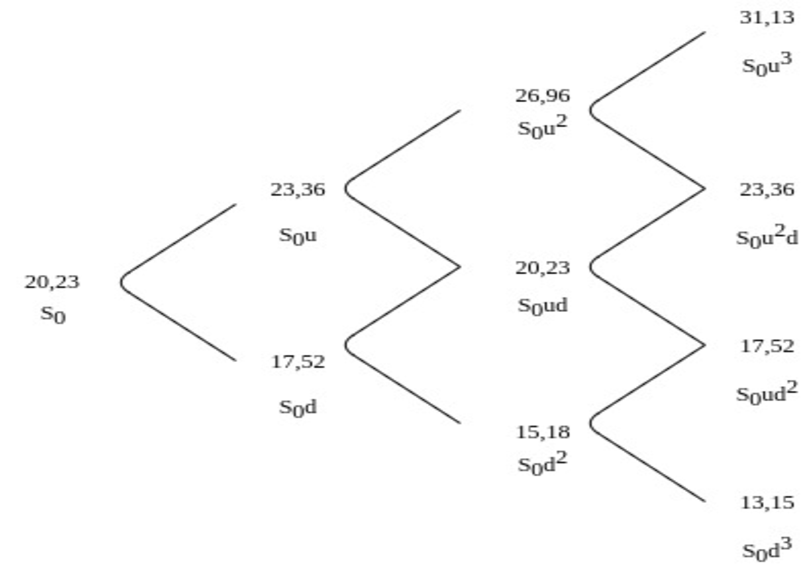
\includegraphics[width=.75\textwidth]{images/eco1.pdf}
% 	\caption{Construção inicial da árvore}
% 	\label{fig:eco1}
% \end{figure}

No entanto, espera-se que o projeto possua duas fases de desenvolvimento. Para isso, foi estabelecido a opção composta sequencial, que ocorre quando um projeto tem múltiplas fases e o andamento para etapas subsequentes dependem necessariamente do sucesso prévio. Realizando os cálculos para a construção dos nós da primeira e segunda etapa, além dos valores estimados com o objetivo de manter ou abandonar o projeto, a análise das opções combinadas pode ser visualizada na Figura \ref{fig:eco2}. 

Os valores presentes líquidos (VPL) dos futuros fluxos de caixa esperados na análise corroboram com os percentuais dos fatores superiores e inferiores. Ademais, a probabilidade de sucesso é alta, visto que a prova de conceito se mostrou viável no âmbito técnico e possui desdobramentos positivos para futuras etapas.

% \begin{figure}[h!]
% 	\centering
% 	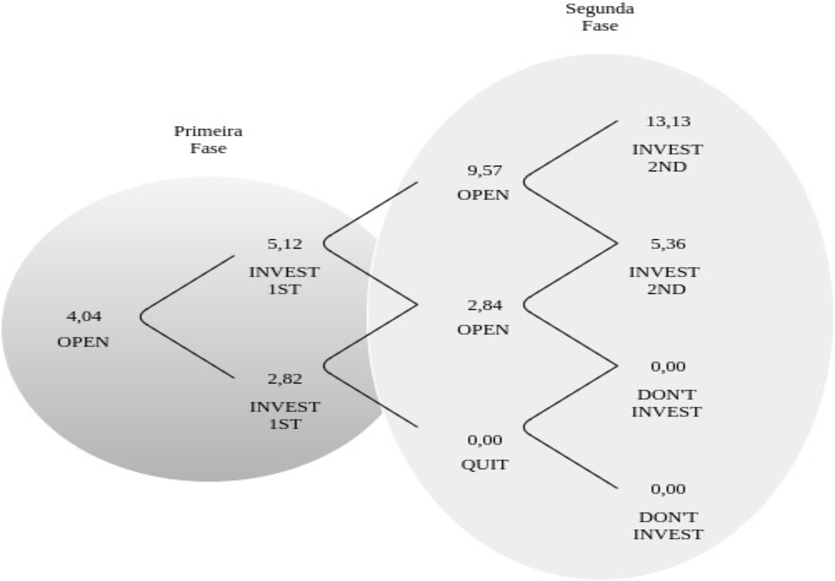
\includegraphics[width=.75\textwidth]{images/eco2.pdf}
% 	\caption{Construção inicial da árvore}
% 	\label{fig:eco2}
% \end{figure}

A resposta positiva à primeira fase, apresentada nos valores do primeiro nó, abrem a possibilidade de investimentos para uma segunda fase de desenvolvimento. Mesmo em um cenário mais desfavorável, os futuros fluxos de caixa possuem valores acima das etapas anteriores, o que demonstra uma gradativa evolução tanto do ponto de vista financeiro quanto técnico, no que diz respeito à apropriação da tecnologia de automação dos manipuladores.

Na segunda fase, apesar de apresentar a metade dos nós com VPL maiores que zero, o cenário é positivo para novas concessões com a propriedade intelectual gerada pelo projeto de P\&D em questão. Além disso, é importante reforçar que as árvores não se utilizaram de futuros fluxos de caixa e nem dos investimentos provenientes do monitoramento sísmico (\textit{nodes all-in-two}), o que poderia gerar externalidades positivas ainda mais significativas, uma vez que a empresa detém a apropriabilidade tecnológica dos nodes. 

Em síntese, é possível inferir que há retornos significativos com os esforços de P\&D a serem realizados nos períodos subsequentes. Evidentemente que a análise de Opções Reais possui limitações, como não considerar riscos associados a grandezas macroeconômicas, ou levar em consideração a volatilidade como uma constante ao longo do tempo. Porém, diante dos cenários apresentados e da capacidade de apropriação sobre a tecnologia, o horizonte para exploração de novas oportunidades sobre automação dos manipuladores submarinos é favorável.


%---- Conclusão ----------------------
\section{Conclusão análise econômica}
\label{sec:rskdesen}

A partir das análises efetuadas neste estudo, e do ponto de vista econômico, pode-se concluir que as hipóteses levantadas - reduções de custo de inspeção e intervenções com manipuladores de ROV, e ganhos de performance associados ao tempo de execução - foram corroboradas pelas significativas reduções tanto no tempo dos conjuntos de atividades quanto nos custos associados à realização destas, que apresentam valores entre 50 e 75\% dos desempenhos atuais com os condutores. 

Verificando o processo de valoração do projeto de P\&D em questão, o cenário é favorável para que se realize novos esforços inovativos, uma vez que será possível não somente apropriar-se da tecnologia disruptiva como também dos lucros monopolísticos associados à concessão da propriedade intelectual para terceiros, que, no melhor cenário possível, pode chegar a 3,25 vezes o VPL apresentado no início do projeto. 

Ao levar em consideração os custos associados com o monitoramento sísmico, as estimativas de redução são ainda mais otimistas se comparadas às atividades mais tradicionais realizadas com os manipuladores, ficando entre 57,14 e 63,64\% comparando com os valores sem automação. 

Por fim, faz-se uso de algumas possíveis recomendações para futuros desdobramentos destes estudos, como a valoração do projeto de monitoramento sísmico, avaliação \textit{ex-post} dos ganhos associados à automação dos manipuladores de ROV, e os possíveis desdobramentos com as oportunidades tecnológicas futuros no tema. 

	%=========================================================
%---- fase design desenvolvimento & testes ---------------
%=========================================================
\chapter{ABRANGÊNCIA DO HARDWARE}
\label{chap:abrhw}

%---- fase design ----------------------------------------
\section{Modelo esquemático de comunicação e elétrica}
\label{sec:modesq}

%---- fase design ----------------------------------------
\section{Arquitetura eletro-eletrônica}
\label{sec:arqelet}

%---- fase design ----------------------------------------
\section{Arquitetura mecânica}
\label{sec:arqmec}

%---- fase design ----------------------------------------
\section{Requisitos de hardware}
\label{sec:reqhw}

%---- fase design ----------------------------------------
\section{\textit{Datasheet} dos componentes}
\label{sec:dtcomp}

%---- fase design ----------------------------------------
\subsection{Lista dos componentes}
\label{sec:lstcomp}

%---- fase design ----------------------------------------
\subsection{Componente A}
\label{sec:comp-a}

%---- fase design ----------------------------------------
\section{Análise dos modos e efeitos de falhas}
\label{sec:hwfmeca}

%---- fase design ----------------------------------------
\section{Análise da árvore de falhas}
\label{sec:hwfta}

%---- fase design ----------------------------------------
\section{Esquemas mecânicos}
\label{sec:esqmec}

%---- fase design ----------------------------------------
\section{Esquemas elétricos}
\label{sec:esqelet}

%---- fase design ----------------------------------------
\section{Esquemas eletrônicos}
\label{sec:esqele}

%---- fase desenvolvimento & testes ----------------------
\section{Produção e montagem}
\label{sec:prodmont}



	%=========================================================
%---- fase design desenvolvimento & testes conclusão -----
%=========================================================
\chapter{ABRANGÊNCIA DO SOFTWARE}
\label{chap:abrsw}

%---- fase design ----------------------------------------
\section{Arquitetura de software}
\label{sec:arqsw}

%---- fase design ----------------------------------------
\section{Requisitos de software}
\label{sec:reqsw}

%---- fase design ----------------------------------------
\section{Diagrama de componentes}
\label{sec:diagcomp}

%---- fase desenvolvimento & testes ----------------------
\section{Matriz de rastreabilidade de testes}
\label{sec:matrtest}

%---- fase desenvolvimento & testes ----------------------
\section{Plano de testes}
\label{sec:plantest}

%---- fase desenvolvimento & testes ----------------------
\section{Integração do sistema}
\label{sec:intsist}

%---- fase conclusão -------------------------------------
\section{Diagrama de classes}
\label{sec:diagclas}

%---- fase conclusão -------------------------------------
\section{Diagrama de sequência}
\label{sec:diagseq}



	%%=========================================================
%---- fase desenvolvimento & testes conclusão ------------
%=========================================================
\chapter{ABRANGÊNCIA DE CONFIABILIDADE}
\label{chap:abrconf}

%---- fase desenvolvimento & testes ----------------------
\section{Diagrama de blocos de Confiabilidade (RBD)}
\label{sec:rbd}

%---- fase conclusão -------------------------------------
\section{Análise dos modos e efeitos de falhas}
\label{sec:conffmeca}

%---- fase conclusão -------------------------------------
\section{Análise da árvore de falhas}
\label{sec:conffta}

%---- fase conclusão -------------------------------------
\section{Análise bayesiana}
\label{sec:bayes}



	%%=========================================================
%---- fase design ----------------------------------------
%=========================================================
\chapter{ESPECIFICAÇÃO DA INTERFACE}
\label{chap:espint}



	%%=========================================================
%---- fase todas -----------------------------------------
%=========================================================
\chapter{TESTES}
\label{chap:testes}

%---- fase conceitual ------------------------------------
\section{Testes conceituais}
\label{sec:tstconc}

%---- fase design ----------------------------------------
\section{Testes em laboratório}
\label{sec:tstlab}

%---- fase desenvolvimento & testes ----------------------
\section{Testes de campo}
\label{sec:tstcamp}

%---- fase conclusão -------------------------------------
\section{Demonstração}
\label{sec:tstconcl}



	%%=========================================================
%---- fase todas -----------------------------------------
%=========================================================
\chapter{AVALIAÇÃO DA PRONTIDÃO TECNOLÓGICA}
\label{chap:trl}



\begin{table}[!h]
\caption{Information on Swiss nuclear power plants}
  \begin{threeparttable}[t]
  \centering
       \begin{tabular}{lrlrrr}
    \toprule
     Reactor     & Initial operation & Type  & Capacity (MW) & Possible Closure\tnote{1}\\
    \midrule
    Beznau I & 17.07.1969 & Pressurised water reactor & 365   & 2029 \\
    Beznau II & 23.10.1971 & Pressurised water reactor & 365   & 2031 \\
    Mühleberg & 01.07.1971 & Boiling water reactor & 373   & 2019\tnote{2}\\
    Gösgen & 02.02.1979 & Pressurised water reactor & 1010  & 2039 \\
    Leibstadt & 24.05.1984 & Boiling water reactor & 1220  & 2044 \\
     \bottomrule
  \end{tabular}
     \begin{tablenotes}
     \item[1] Assumption: life time of 60 years.
     \item[2] Official shut-down.
   \end{tablenotes}
    \end{threeparttable}%
  \label{tab:addlabel}%
\end{table}%

%---- fase conceitual ------------------------------------
\section{Fase conceitual}
\label{sec:trlconc}

%---- fase design ----------------------------------------
\section{Fase design}
\label{sec:trldesig}

%---- fase desenvolvimento & testes ----------------------
\section{Fase desenvolvimento}
\label{sec:trldesen}

%---- fase conclusão -------------------------------------
\section{Fase final}
\label{sec:trlconcl}

%---- fase conclusão -------------------------------------
\section{Avaliação da matriz tecnológica do sistema}
\label{sec:avaltec}



	\chapter{ANÁLISE ECONÔMICA}
\label{chap:rskk}

%---- Análise de custos das operações com ROV ------------------------------------
\section{Análise de custos}
\label{sec:rskconc}
Os custos com operações offshore receberam limitada atenção dos meios acadêmico e corporativo. Em boa parte, os custos com a produção com petróleo e gás ocupam uma pequena porção orçamentária, além dos altos preços das commodities gerarem grandes fluxos de caixa, aumentando a produção e vendas por consequência \cite{kaiser2019role}.

Diferente dos custos de capital para prospecção de petróleo e seus derivados, os custos operacionais são menos transparentes , com menor disponibilidade de dados e informações pertinentes para avaliação, vindo de diferentes formas e aplicações. Apesar de tais obstáculos, há estudos de benchmark que propuseram diminuir o gap entre as informações obtidas e a avaliação resultante do processo, obtendo relativo êxito em suas execuções. 

A proposta desta seção é avaliar os custos associados ao uso de manipuladores subaquáticos em ROVs. Para isso, os dados foram coletados e utilizados segundo informações da Petrobras a cerca dos contratos de embarcação de ROV para inspeção, reparo e manutenção, conforme apresentado na Tabela \ref{tab:cost1}:

\begin{table}[h]
	\centering
	\begin{threeparttable}
	\centering
	\caption{Variáveis de embarcação tipo RSV}
	\label{tab:cost1}
	\begin{tabular}{p{8cm} >{\centering\arraybackslash}m{3.7cm}}
		\hline
		\multicolumn{1}{c}{\textbf{Variáveis}} & \textbf{Valores}\tnote{i}  \\ \hline
		Diária RSV                              & US\$81.474,45     \\
		Ciclo 28 dias                          & US\$2.281.284,60  \\
		Total contrato RSV                     & US\$44.667.552,47 \\
		Total dias de contrato                 & 547               \\
		                                       &                   \\
		Total de operações (A)\tnote{ii}       & 1976              \\
		Total de inspeções                     & 1337              \\
		Total de intervenções                  & 639               \\
		Número de anomalias (B)                & 432               \\
		Índice de anomalias (B/A)              & 21,86\%           \\ \hline
	\end{tabular}
\begin{tablenotes}
\item Fonte: Petrobras. Elaboração dos autores.
\item[i]{Valores monetários a US\$ correntes}
\item[ii]{Operações e anomalias tiveram seus valores projetados para um ciclo contratual de 547 dias.}
\end{tablenotes}
\end{threeparttable}
\end{table}


Pode-se observar que os contratos de embarcação tipo RSV (ROV Support Vessel) da Petrobras são realizados em ciclos de 28 dias\footnote{Há também outros contratos internacionais que estabelecem um dia útil de 12 horas de trabalho, com permissão máxima de inatividade do ROV de 30 horas por mês \cite{kaiser2019role}.} , com 1 dia de manutenção e reparo de equipamentos, alcançando a diária aproximada de US\$ 81 mil\footnote{Alguns estudos empíricos registram taxas diárias para RSV entre 100 e 300 mil dólares, dependendo do tamanho da embarcação utilizada.}. O valor da diária inclui, além do afretamento, materiais, equipamentos, bens importados e tripulação. 

Para gerar efeitos comparativos mais precisos, e considerando o uso da embarcação por 24 horas, as atividades descritas nos conjuntos da Tabela \ref{tab:cost2} terão o valor da diária estabelecido em minutos. A ideia consiste em mensurar a participação de uma determinada atividade em relação ao total previsto em um dia completo de operações. 
Estabeleceu-se a divisão das operações por conjunto segundo o nível de complexidade inerente à sua realização, i.é., o Conjunto 1 pode demandar um tempo menor de execução se comparado aos Conjuntos 3 e 4, por exemplo. As médias apresentadas na tabela seguem a seguinte estrutura:

\begin{itemize}
	\item Frequência média mensal auferida por cada atividade registrada pela Petrobras;
	\item Tempo médio de execução de cada atividade registrada pela Petrobras no período vigente sem automação dos manipuladores;
	\item Tempo esperado, em média, com a automação dos manipuladores para realizar os conjuntos de atividades.
\end{itemize}

\begin{table}[h]
	\renewcommand{\arraystretch}{1.2}
    \centering
    \resizebox{\textwidth}{!}{
	\begin{threeparttable}
	\centering
	\caption{Variáveis de embarcação tipo RSV}
	\label{tab:cost2}
    \begin{tabular}{l >{\centering\arraybackslash}m{3.0cm} >{\centering\arraybackslash}m{3.0cm} >{\centering\arraybackslash}m{3.0cm}}
		\hline
        \textbf{Operação submarina\tnote{i}}           & \textbf{Frequência média mensal} & {\textbf{Sem automação (min)}} & \textbf{Com automação (min)} \\ \hline
		Conjunto 1                                     &                                  &                                &                              \\
		\hspace{3mm}Abertura e fechamento de válvulas  & 12                               & 10                             & 5                            \\
		\hspace{3mm}Colocação e retirada de hot stab   & 28                               & 10                             & 4                            \\
		\hspace{3mm}Uso de torque tool                 & 12                               & 15                             & 5                            \\
		Conjunto 2                                     &                                  &                                &                              \\
		\hspace{3mm}Instalação de \textit{tree cap}    & 5                                & 60                             & 30                           \\
		\hspace{3mm}Conexão de \textit{flying leads}   & 10                               & 60                             & 15                           \\
		Conjunto 3                                     &                                  &                                &                              \\
		\hspace{3mm}Limpeza de \textit{hub}\tnote{ii}  & 5                                & 240                            & 60                           \\
		Conjunto 4                                     &                                  &                                &                              \\
		\hspace{3mm}Instalação de flanges              & 5                                & 180                            & 60                           \\ \hline
	\end{tabular}
	\begin{tablenotes}
		\item Fonte: Petrobras. Elaboração dos autores.
        \item[i]{Foram consideradas duas instalações de ANM por mês com embarcação}
        \item[ii]{Considerou-se somente o tempo de limpeza de um \textit{hub}, uma vez que o tempo de execução registrados possui grandes variações (de horas a dias).}
    \end{tablenotes}
    \end{threeparttable}
    }
\end{table}

A hipótese central para os valores presentes no item C está em aproximar mais precisamente os tempos de execução das atividades presentes nos registros dos melhores condutores dos manipuladores. Por mais que estes tenham a experiência para uma boa condução, ainda há fatores (sejam eles de caráter endógeno ou exógeno) que possibilitam a presença de anomalias, enquanto com a automação estas seriam minimizadas.

O conjunto 1 corresponde às atividades que envolvem acionamento mecânico de válvulas submarinas com o ROV equipado com ferramentas de torque (\textit{torque tool}). Tal conjunto relaciona-se com os demais porque estes dependem diretamente do acionamento de válvulas para que ocorra a instalação/desinstalação de determinados equipamentos, o que justifica a maior frequência de manuseios de válvulas e \textit{torque tools}. Apesar de a Petrobras estabelecer máximo de 15 minutos para movimentos envolvendo válvulas, há registros apontando para valores médios de 10 minutos, com aproximação da média com automação em 5 minutos, uma diminuição de aproximadamente 50\% em relação à média máxima esperada em contrato.

O lançamento/instalação de \textit{Tree Cap} em árvore de natal molhada (ANM) e manuseio de \textit{flying leads}, utilizando ferramenta de torque, compõem o conjunto 2 de serviços do ROV. O principal diferencial para diminuição do tempo de execução em \textit{flying leads} está na presença de uma ferramenta de orientação inserida (FLOT) no ROV para colocá-los na ANM, que pode chegar em até 1/3 do valor comparado ao FLOT não residente. Para fins didáticos, o estudo propôs trabalhar somente com os valores onde há a utilização da ferramenta de orientação, registrando um total de execução de 60 minutos entre instalação e desinstalação dos componentes.

A operação de limpeza de \textit{hubs}, atividade fundamental do Conjunto 3, consiste em remover incrustações e/ou vidas marinhas dos equipamentos a partir de ferramentas de limpeza operadas por ROVs a fim de permitir instalação de subequipamentos. Em certas ocasiões, a limpeza do \textit{hub} está associada à necessidade de retirar as capas de proteção ou capas de teste. Por este motivo, quando realizadas no mesmo período programado, desinstalações de \textit{tree caps} (Conjunto 2) podem interferir diretamente no tempo de execução da limpeza do \textit{hub}, apresentando a maior média de tempo dentre todos os conjuntos de atividades no estudo. Ademais, a atividade em si depende muito da experiência do condutor do ROV e, dentro dos relatos da Petrobras, possui as maiores probabilidades de apresentar anomalias, gerando maiores desvios padrões em relação à média observada. Os valores representados na Tabela 1 para tal conjunto são equivalentes ao tempo médio de somente a realização da limpeza (4 horas aproximadamente).  

Por fim, o Conjunto 4 consiste na instalação de flanges cego (ou cubo cego \textit{grayloc}\footnote{Tecnologia desenvolvida por Oceaneering. Para mais informações, ver: https://www.oceaneering.com/grayloc-technology (acesso em 29/10/2019).}) em conexões de dutos rígidos e flexíveis, a partir de materiais fornecidos pela Petrobras. O conjunto envolve preparação e manuseio do flange no convés, lançamento, instalação de estojos, torqueamento e teste de estaqueidade. Dentro das atividades previstas, a instalação de estojos é a que possui maior interdependência entre os outros conjuntos de atividades descritas anteriormente, envolvendo inspeção visual, limpeza, destorqueamento, medição de potencial eletroquímico, instalação e torqueamento do novo estojo. 

Desta forma, torna-se mais complexa\footnote{Parte dessa complexidade também diz respeito ao uso correto da ferramenta, que deve possuir \textit{handles} em múltiplas posições para facilitar o manuseio pelo manipulador do ROV.}  a mensuração da performance. Para este estudo, a média de tempo para execução adotada foi de 180 minutos, podendo apresentar o mesmo comportamento observado no Conjunto 3.  

Dada a apresentação da estrutura dos conjuntos de atividades com manipuladores de ROV, deu-se prosseguimento à conversão dos dados em unidades monetárias para mensurar as proporções desses custos em relação à diária da embarcação, considerando para o caso somente as operações de intervenção\footnote{Apesar de haver uso de manipuladores para inspeções para casos de limpeza e medição de potencial eletroquímico, sua mensuração em tempo de execução é mais assertiva em inspeções programadas.}. Essa elaboração pode ser observada na Tabela \ref{tab:cost3}, com os valores aproximados por minuto de uma diária completa de atividades, isto é, 24 horas (ou 1440 minutos) ininterruptas de prestação de serviço. 

\begin{table}[h]
	\renewcommand{\arraystretch}{1.2}
    \centering
    \resizebox{\textwidth}{!}{
	\begin{threeparttable}
	\centering
	\caption{Dados monetários dos conjuntos de atividades em ROV}
	\label{tab:cost3}
	\begin{tabular}{l >{\centering\arraybackslash}m{3.0cm} >{\centering\arraybackslash}m{3.0cm} >{\centering\arraybackslash}m{3.0cm}}
			\hline
			\textbf{Operação submarina}                        & \textbf{Valor médio de execução (US\$) (A)\tnote{i}} & \textbf{Valor esperado com automação (B)\tnote{i}} & \textbf{$\Delta$A/B (\%)} \\ \hline
			Conjunto 1                                            &                   &                   &                \\
			\hspace{3mm}Abertura e fechamento de válvulas         & 6.789,54          & 3.394,77          & 50\%           \\
			\hspace{3mm}Colocação e retirada de \textit{hot stab} & 15.842,25         & 6.336,90          & 60\%           \\
			\hspace{3mm}Uso de \textit{torque tool}               & 10.184,31         & 3.394,77          & 67\%           \\
			Conjunto 2                                            &                   &                   &                \\
			\hspace{3mm}Instalação de \textit{tree cap}           & 16.973,84         & 8.486,92          & 50\%           \\
			\hspace{3mm}Conexão de \textit{flying leads}          & 33.947,69         & 8.486,92          & 75\%           \\
			Conjunto 3                                            &                   &                   &                \\
			\hspace{3mm}Limpeza de \textit{hub}                   & 67.895,38         & 16.973,84         & 75\%           \\
			Conjunto 4                                            &                   &                   &                \\
			\hspace{3mm}Instalação de flanges                     & 50.921,53         & 16.973,84         & 67\%           \\ \hline
	\end{tabular}
	\begin{tablenotes}
		\item Fonte: Petrobras. Elaboração dos autores.
		\item [i]Valores em US\$ a preços correntes.
	\end{tablenotes}
	\end{threeparttable}
	}
\end{table}
Observando os dados oriundos da Tabela \ref{tab:cost3}, nota-se que as argumentações anteriormente apresentadas corroboram com os valores monetários expressos, sobretudo na interdependência dos Conjuntos 3 e 4 em relação às atividades mais ordinárias. É evidente que os dados apresentem proporções diretas com o presente na Tabela \ref{tab:cost2}, visto que foram multiplicados por um valor constante (valor da diária de embarcação por minuto), o que justifica as variações percentuais entre 50 e 75\% das médias sem e com intermédio da automação, respectivamente.

Ademais, pode-se esperar margens ainda maiores com as atividades que possuem tempos de execução com alto desvio-padrão, como é o caso da instalação de \textit{tree cap} e da limpeza de \textit{hub}. 

Ao realizar a soma dos valores monetários dos conjuntos, obtêm-se algumas importantes observações e desdobramentos, que podem ser verificados na Tabela \ref{tab:cost4}.

\begin{table}[h]
	\renewcommand{\arraystretch}{1.2}
	\centering
	\resizebox{\textwidth}{!}{
	\begin{threeparttable}
	\centering
	\caption{Soma dos custos das atividades com manipuladores}
	\label{tab:cost4}
		\begin{tabular}{llll}
			\hline
			\textbf{Conjunto de Operações} & \textbf{Valor sem automação (A)} & \textbf{Valor com automação (B)} & \textbf{Redução (A - B)} \\ \hline
			Conjunto 1                     & 32.816,10                        & 13.126,44                        & 19.689,66                \\
			Conjunto 2                     & 50.921,53                        & 16.973,84                        & 33.947,69                \\
			Conjunto 3                     & 67.895,38                        & 16.973,84                        & 50.921,53                \\
			Conjunto 4                     & 50.921,53                        & 16.973,84                        & 33.947,69                \\
			\textbf{Total}                 & \textbf{202.554,54}              & \textbf{64.047,97}               & \textbf{138.506,57}      \\ \hline
		\end{tabular}
		\begin{tablenotes}
			\item Fonte: Petrobras. Elaboração dos autores.
			\item [i]Valores em US\$ a preços correntes.
	\end{tablenotes}
	\end{threeparttable}
	}
\end{table}

Com os valores monetários expressos na Tabela \ref{tab:cost4}, espera-se que haja uma redução de custos de aproximadamente 59\%  \footnote{O percentual não englobou os custos associados a pessoal e logística, assim como a depreciação, reparos e manutenções necessárias.}em relação aos conjuntos de operações realizados sem automação. Visto que são valores representativos a duas instalações simultâneas em árvores de natal molhada por mês, esses podem obter um impacto ainda mais significativo se analisado em período anual.

Além dos impactos diretos nos custos com as operações dos manipuladores, outros possíveis efeitos indiretos devem ser considerados como, por exemplo, a minimização de anomalias em riscos ambientais e diminuição do consumo de óleo diesel, necessário para o funcionamento das embarcações de ROVs. 

Por fim, vale destacar a importância de um conjunto de atividades específicas ao monitoramento sísmico marítimo utilizando receptores pontuais (também conhecidos como \textit{nodes}). 

Por ser uma tecnologia disruptiva, pioneira no âmbito mundial, ela servirá para gerenciamento da produção dos reservatórios do Pré-Sal da Bacia de Santos. As hipóteses para sua implementação são os ganhos de qualidade intrínseca dos dados sísmicos - incluindo qualidade sísmica 4D - e ganhos de tempo de processamento destes dados. Além da maior flexibilidade operacional e qualidade dos dados, o conceito terá uma rápida capacidade de apropriação pela Petrobras, uma vez que a tecnologia já está madura e amplamente desenvolvida na empresa\footnote{Um exemplo desse domínio são as estacas-torpedos, empregadas como meio de baixo custo para enterramento dos \textit{nodes}.}.

As etapas previstas para as quais a tecnologia deverá passar são: 

\begin{itemize}
	\item Prototipagem, que inclui a produção de uma maquete em escala reduzida;
	\item Validação dos componentes e do sistema em escala laboratorial, ainda na fase de P\&D;
	\item Testes em escala reduzida, ambiente controlado e incluindo a estaca instrumentada;
	\item Produção de cinco unidades constituídas de um Módulo Submarino de Aquisição de Dados Sísmicos (MSADS) e um Dispositivo de Transporte e Liberação de Estacas (DLTE);
	\item Teste de campo para validação da operação em condições realistas;
	\item Avaliação da prova de conceito final e recomendações para manufatura em escala comercial.
\end{itemize}

A justificativa para tal conceito estar dentro do estudo encontra-se nas operações do ROV com o Módulo de Estaca-Suporte (MES), MSADS, Módulo de Posicionamento e Alinhamento (MPA), sendo estas necessárias tanto para operações de instalação quanto de desinstalação dos componentes, cujos tempos de execução sem a automação e os previstos com a implementação da automação dos manipuladores podem ser observados na Tabela \ref{tab:node1}.

\begin{table}[h]
	\renewcommand{\arraystretch}{1.2}
	\centering
	\resizebox{\textwidth}{!}{
	\begin{threeparttable}
	\centering
	\caption{Tempos de execução com operações do MSADS}
	\label{tab:node1}
		\begin{tabular}{l >{\centering\arraybackslash}m{3.0cm} >{\centering\arraybackslash}m{3.0cm} >{\centering\arraybackslash}m{3.0cm}}
			\hline
			\textbf{}                                                                      & \multicolumn{2}{c}{\textbf{Duração}}                   \\ \hline
			\textbf{Etapa/Descrição}                                                       & \textbf{Manual (min)}                       & \textbf{Automático (min)}      \\ \hline
			Instalação                                                                     &                                             &          \\
			\hspace{3mm}Posicionar o MSADS no disco da estaca                              & 12                                          & 5        \\
			\hspace{3mm}Retirar capa protetora do conector elétrico e colocá-la no suporte & 14                                          & 6        \\
			\hspace{3mm}Retirar conector elétrico no jumper e colocar em painel de estaca  & 15                                          & 6        \\
			Desinstalação                                                                  &                                             &          \\
			\hspace{3mm}Desconectar do jumper do painel e colocar o conector elétrico      & 12                                          & 5        \\
			\hspace{3mm}Recolocar a capa protetora no painel de estaca                     & 14                                          & 6        \\
			\hspace{3mm}Retirar o MSADS do disco da estaca                                 & 11                                          & 4        \\ \hline
		\end{tabular}
		\begin{tablenotes}
			\item Fonte: Petrobras. Elaboração dos autores.
		\end{tablenotes}
	\end{threeparttable}
	}
\end{table}

As etapas das operações que necessitam do auxílio do ROV consistem em lançar várias estacas-suporte em ambiente submarino, conectar os módulos permanentes e não-permanentes, registro sísmico, desconexão do módulo de eletrônica e recuperação dos dados registrados.  

O MSADS, também conhecido como Módulo de Eletrônica, contém um suporte para que este seja suspenso por um ROV, além de um conector de conexão molhada, manuseável pelo manipulador presente no veículo, para colocá-lo ao painel da Estaca-suporte. 

Inicialmente posiciona-se o MSADS no disco de estaca, procedimento que leva em média 12 minutos para execução. Em seguida, retira-se a capa protetora do conector elétrico no painel da estaca e coloca essa em seu suporte no painel, com uma estimativa de execução de aproximadamente 14 minutos. Compondo a etapa final de instalação, há a retirada do conector elétrico na extremidade do \textit{jumper}\footnote{Operações de conexões e desconexões de \textit{jumper} elétrico consistem em realizar interligações/desconexões elétrica entre equipamentos e/ou subequipamentos submarinos com a finalidade de permitir comando e monitoramento eletroeletrônico a partir da superfície.}  no MSADS e realiza-se a conexão deste no painel da estaca, com tempo estimado de 15 minutos para realização. Espera-se que, com a automação dos manipuladores, haja uma redução média de 24 minutos entre todas as operações de instalação.

Para os processos de desinstalação, de início, a primeira etapa consiste em desconectar o \textit{jumper} do painel da estaca e colocar o conector elétrico do \textit{jumper} em seu suporte no Módulo de Eletrônica, com duração aproximada de 12 minutos. A etapa seguinte procura recolocar a capa protetora no conector elétrico do painel da Estaca-suporte, levando em média 14 minutos para sua execução. Por fim, realiza-se a operação de retirada do MSADS do disco de estaca por volta de 11 minutos. Da mesma maneira que nas instalações, com a automação espera-se que haja uma redução total cerca de 22 minutos.

\begin{table}[h]
	\renewcommand{\arraystretch}{1.2}
	\centering
	\resizebox{\textwidth}{!}{
	\begin{threeparttable}
	\centering
	\caption{Valores das atividades realizadas com nodes}
	\label{tab:node2}
		\begin{tabular}{l >{\centering\arraybackslash}m{3.0cm} >{\centering\arraybackslash}m{3.0cm} >{\centering\arraybackslash}m{3.0cm}>{\centering\arraybackslash}m{3.0cm}}
			\hline
			\textbf{}                                                & \multicolumn{3}{c}{\textbf{Valores (diária)}}   \\ \hline
			\textbf{Etapa/Descrição}                                 & \textbf{Manual (US\$) (A)} & \textbf{Automático (US\$) (B)} & \textbf{A/B(\%)} \\ \hline
			Instalação                           							   &                                                                       &                           &                                         \\
			\hspace{3mm}Posicionamento do MSADS no disco da estaca             & 1.250,00                                                              & 520,83                    & 58,33                                   \\
			\hspace{3mm}Retirar e colocar capa protetora do conector elétrico  & 1.458,33                                                              & 625,00                    & 57,14                                   \\
			\hspace{3mm}Retirar e colocar conector elétrico no jumper          & 1.562,50                                                              & 625,00                    & 60,00                                   \\
			Desinstalação                                                      &                                                                       &                           &                                         \\
			\hspace{3mm}Desconectar do jumper e colocar o conector elétrico    & 1.250,00                                                              & 520,83                    & 58,33                                   \\
			\hspace{3mm}Recolocar a capa protetora no conector elétrico        & 1.458,33                                                              & 625,00                    & 57,14                                   \\
			\hspace{3mm}Retirar o MSADS do disco da estaca                     & 1.145,83                                                              & 416,67                    & 63,64                                   \\ \hline
		\end{tabular}%
		\begin{tablenotes}
			\item Fonte: Petrobras. Elaboração dos autores.
			\item [i]Valores em US\$ a preços correntes.
		\end{tablenotes}
	\end{threeparttable}
	}
\end{table}
De maneira análoga ao apresentado nas Tabelas \ref{tab:cost3} e \ref{tab:cost4}, os dados dos tempos de execução em operações com os módulos submarinos foram multiplicados por um valor da diária de embarcação proporcional por minuto. Para operações como essas, a embarcação mais adequada é a de pesquisa sísmica, cujo valor adotado foi de US\$161,9 mil\footnote{Tanto em relatórios anuais das empresas prestadoras de serviços quanto a literatura acadêmica empírica utilizam de uma margem que, para os valores correntes, chegam entre US\$150 e US\$200 mil.} , e que pode ser observado na Tabela \ref{tab:node2}. 

As variações percentuais presentes na última coluna corroboram a importância da automação nos processos envolvendo monitoramento sísmico\footnote{Vale ressaltar que a instalação do Módulo de Posicionamento e Alinhamento (MPA) também pode ser autônomas. Para tal, espera-se que haja uma redução de 2 minutos, em média, entre as operações sem e com automação. Por ser uma oportunidade tecnológica em fase de exploração pela Petrobras, não há dados monetários concretos para serem levantados.}. Por   permanente. Os valores monetários expressos podem ainda sofrer alterações significativas dependendo da diária estabelecida em contrato, dentro dos padrões internacionais para este tipo de atividade. Quando representados em um período contratual de uma embarcação de pesquisa sísmica, as operações elucidadas na Tabela \ref{tab:node3} possuem amplas margens de redução de custo com a automação.

\begin{table}[h]
	\renewcommand{\arraystretch}{1.2}
	\centering
	\resizebox{\textwidth}{!}{
	\begin{threeparttable}
	\centering 
	\caption{Valores proporcionais em período de contratação - nodes}
	\label{tab:node3}
		\begin{tabular}{lllll}
			\hline
			\multicolumn{1}{c}{\textbf{Tipo de operação}} & \multicolumn{1}{c}{\textbf{\begin{tabular}[c]{@{}c@{}}Manual (US\$ 1000) \\ mín\tnote{ii}\end{tabular}}} & \multicolumn{1}{c}{\textbf{\begin{tabular}[c]{@{}c@{}}Automático (US\$ 1000) \\ mín\end{tabular}}} & \multicolumn{1}{c}{\textbf{\begin{tabular}[c]{@{}c@{}}Manual (US\$ 1000) \\ máx\tnote{iii}\end{tabular}}} & \multicolumn{1}{c}{\textbf{\begin{tabular}[c]{@{}c@{}}Automático (US\$ 1000) \\ máx\end{tabular}}} \\ \hline
			Instalação                                    & 4.609,47                                                                                       & 1.911,24                                                                                           & 27.656,81                                                                                      & 11.467,46                                                                                          \\
			Desinstalação                                 & 4.159,76                                                                                       & 1.686,39                                                                                           & 24.958,58                                                                                      & 10.118,34                                                                                          \\
			\textbf{Total}                                & \textbf{8.769,23}                                                                              & \textbf{3.597,63}                                                                                  & \textbf{52.615,39}                                                                             & \textbf{21.585,80}                                                                                 \\
			\textbf{Diferença}                            & \textbf{-}                                                                                     & \textbf{5.171,60}                                                                                  & \textbf{-}                                                                                     & \textbf{31.029,59}                                                                                 \\ \hline
		\end{tabular}%
		\begin{tablenotes}
			\item Fonte: Petrobras. Elaboração dos autores.
			\item [i]Valores em US\$ milhares a preços correntes.
			\item [ii]Valores mínimos para um ciclo contratual operando em 1000 \textit{nodes}.
			\item [iii]Valores máximos para um ciclo contratual operando em 6000 \textit{nodes}.
		\end{tablenotes}
	\end{threeparttable}
	}
\end{table}

Quando agregadas as atividades de instalação e desinstalação dos Módulos de Eletrônica, a redução de custo pode variar de 5,2 a 31 milhões de dólares por contrato. A justificativa para o desvio padrão apresentado está na quantidade de intervenções já realizadas até então pela Petrobras por ciclos contratuais. Ademais, tal desvio padrão viabiliza as oportunidades tecnológicas presentes na automação do monitoramento sísmico, com o escopo de 2 anos e meio para tornar o sistema no mínimo semi-operacional.

Em suma, do ponto de vista financeiro, espera-se que a automação provenha reduções significativas de custos associadas aos manipuladores de ROV, seja em operações mais ordinárias, como aberturas e fechamentos de válvulas, seja em operações onde a Petrobras obterá o pioneirismo mundial, como nas operações de intervenções em \textit{nodes all-in-two}. 

Entretanto, para que a automação dos manipuladores seja considerada viável no âmbito econômico, verificou-se a necessidade de se avaliar a rentabilidade dos projetos de P\&D associados, em uma metodologia de valoração amplamente utilizada por empresas e academia, e que será explorada na seção seguinte. 


%---- Modelo de Valoração P&D ----------------------------------------
\section{Modelo de valoração dos projetos de P\&D}
\label{sec:rskdesig}

A fim de obterem vantagens competitivas que proporcionem lucros monopolísticos\footnote{A busca de oportunidades ou inovação, em seu sentido mais amplo, geram monopólios temporários, de menor ou maior período, até que sejam desafiados por novos concorrentes ou imitadores, tornando a concorrência um processo ativo e evolutivo de espaço e oportunidades tecnológicos. Para mais, ver \cite{possas2002concorrencia}.} , as empresas buscam inovações e o mercado, consequentemente, selecionam os resultados econômicos oriundos dessas mesmas inovações através de decisões estratégicas. 

Essas estratégias podem ocorrer através de investimentos em P\&D, atuando como ativos intangíveis e cujos esforços convertem-se em desenvolvimento de novos produtos, processos e/ou serviços. Os resultados deste processo são observáveis através dos impactos gerados na esfera empresarial, ou até mesmo no âmbito socioeconômico. 

No entanto, como discutido na introdução, os esforços para se investir em P\&D possuem incertezas inerentes que tornam a atividades de difícil avaliação ex-ante. Para isso, a Teoria de Opções Reais apresenta-se como um método robusto para análises de cenários onde há presença de incerteza e flexibilidade gerencial de longo prazo \cite{dixit1994investment}{mun2002real}. 

Considerando que todo projeto de P\&D é, em essência, um projeto de investimento produtivo, este pode ser visto como um conjunto de opções reais. Dentre tais opções, as empresas detêm a capacidade de optar de adiar o investimento, cancelar novas etapas, alterar a escala produtiva (como é o caso de expansão e contração), abandonar por conta do excessivo ônus e opções de crescimento \cite{meirelles2004teoria}. 

Para a construção da análise, utilizaram-se dados provenientes da última demonstração financeira da Petrobras e dos esforços de P\&D, que estarão concentrados integralmente nos recursos alocados e esperados em parceria com o SENAI CIMATEC, e que podem ser observados na Tabela 6.

\begin{table}[h]
	\renewcommand{\arraystretch}{1.2}
	\centering
	\begin{threeparttable}
	\centering
	\caption{Variáveis utilizadas para modelo de valoração}
	\label{tab:valor1}
	\begin{tabular}{p{8cm} >{\centering\arraybackslash}m{3.7cm}}
		\hline
		\multicolumn{1}{c}{\textbf{Variáveis}} & \textbf{Valor} \\ \hline
		Investimento na Fase 1                 & R\$ 1,34 mi    \\
		Investimento na Fase 2\tnote{a}        & R\$ 18 mi      \\
		VPL descontado                         & R\$ 20,23 mi   \\
		Volatilidade\tnote{b}                  & 25\%           \\
		Taxa risk-free                         & 5\%            \\
		Período da Fase 1                      & 1 ano          \\
		Período da Fase 2                      & 2 anos         \\ \hline
	\end{tabular}
	\begin{tablenotes}
		\item Fonte: Petrobras. Elaboração dos autores.
		\item [a]Valores e período estimado para a segunda fase do projeto.
		\item [b]Volatilidade calculada através da simulação Monte Carlo baseado na metodologia AD\textsuperscript{2}
	\end{tablenotes}
\end{threeparttable}
\end{table}

O investimento para o projeto foi dividido em duas grandes fases: inicialmente, o desenvolvimento viável das provas de conceito para, em seguida, testar o desempenho da automação dos manipuladores em ambientes reais. Para isso, estima-se investimentos de aproximadamente R\$ 19,34 milhões em um período de 3 anos. Utilizando a simulação Monte Carlo, e baseado na convergência das respostas dos pesquisadores com a metodologia AD\textsuperscript{2} (Advancement Degree of Difficulty)\footnote{A metodologia baseia-se na mensuração das dificuldades previstas no projeto para amadurecer o uso da tecnologia. Variáveis como custo, cronograma e os riscos inerentes às fases do projeto são consideradas na avaliação.} , a volatilidade implícita dos fluxos de caixa esperados com o projeto é de 25\%. 

Para a valoração estática dos lucros futuros, utilizou-se o modelo de fluxos de caixa descontado por uma taxa de desconto baseada no custo médio ponderado sobre o capital. A partir dos dados provenientes das demonstrações financeiras, a Petrobras teve, em 2018, 290 propriedades intelectuais (em grande parte, patentes) concedidas no Brasil e exterior. O valor adicionado recebido em alugueis, royalties e outros por conta de tais propriedades ficou em torno de R\$1,1 bilhão. Constatando os valores adicionados em períodos anteriores e dividindo pelas patentes concedidas, calculou-se o valor de R\$2,62 milhões por concessão, que serviu para a elaboração dos fluxos de caixa descontados, obtendo o resultado esperado de R\$20,23 milhões. 

O cálculo da árvore inicial é similar às operações tradicionais de opções reais com ativos, calculando os fatores superiores e inferiores e envolvendo o valor presente dos fluxos de caixa futuros para os próximos três anos, presente na Figura \ref{fig:eco1}.

\begin{figure}
	\centering
	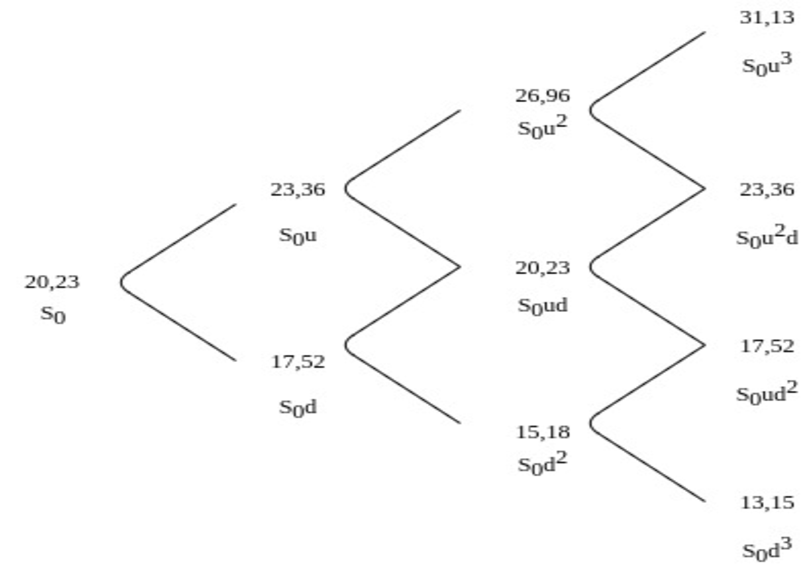
\includegraphics[width=.75\textwidth]{images/eco1.pdf}
	\caption{Construção inicial da árvore}
	\label{fig:eco1}
\end{figure}

No entanto, espera-se que o projeto possua duas fases de desenvolvimento. Para isso, foi estabelecido a opção composta sequencial, que ocorre quando um projeto tem múltiplas fases e o andamento para etapas subsequentes dependem necessariamente do sucesso prévio. Realizando os cálculos para a construção dos nós da primeira e segunda etapa, além dos valores estimados com o objetivo de manter ou abandonar o projeto, a análise das opções combinadas pode ser visualizada na Figura \ref{fig:eco2}. 

Os valores presentes líquidos (VPL) dos futuros fluxos de caixa esperados na análise corroboram com os percentuais dos fatores superiores e inferiores. Ademais, a probabilidade de sucesso é alta, visto que a prova de conceito se mostrou viável no âmbito técnico e possui desdobramentos positivos para futuras etapas.

\begin{figure}[h]
	\centering
	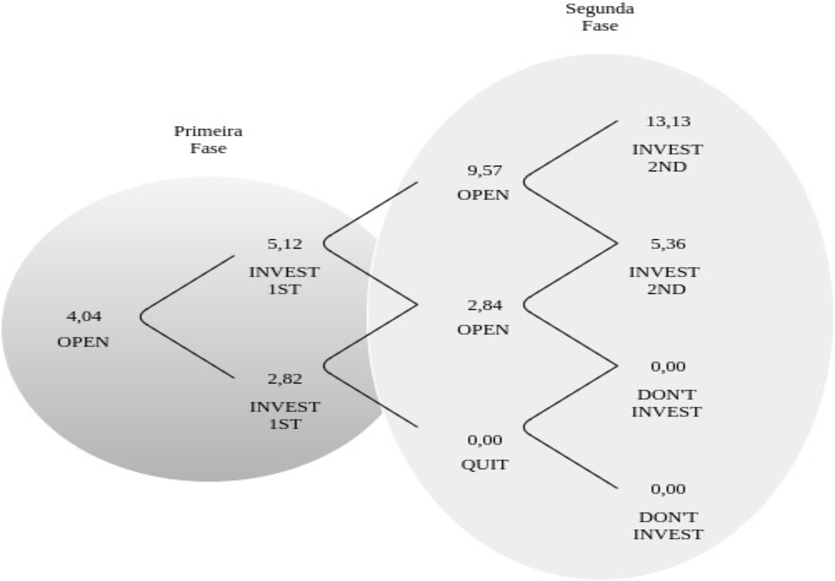
\includegraphics[width=.75\textwidth]{images/eco2.pdf}
	\caption{Construção inicial da árvore}
	\label{fig:eco2}
\end{figure}

A resposta positiva à primeira fase, apresentada nos valores do primeiro nó, abrem a possibilidade de investimentos para uma segunda fase de desenvolvimento. Mesmo em um cenário mais desfavorável, os futuros fluxos de caixa possuem valores acima das etapas anteriores, o que demonstra uma gradativa evolução tanto do ponto de vista financeiro quanto técnico, no que diz respeito à apropriação da tecnologia de automação dos manipuladores.

Na segunda fase, apesar de apresentar a metade dos nós com VPL maiores que zero, o cenário é positivo para novas concessões com a propriedade intelectual gerada pelo projeto de P\&D em questão. Além disso, é importante reforçar que as árvores não se utilizaram de futuros fluxos de caixa e nem dos investimentos provenientes do monitoramento sísmico (\textit{nodes all-in-two}), o que poderia gerar externalidades positivas ainda mais significativas, uma vez que a empresa detém a apropriabilidade tecnológica dos nodes. 

Em síntese, é possível inferir que há retornos significativos com os esforços de P\&D a serem realizados nos períodos subsequentes. Evidentemente que a análise de Opções Reais possui limitações, como não considerar riscos associados a grandezas macroeconômicas, ou levar em consideração a volatilidade como uma constante ao longo do tempo. Porém, diante dos cenários apresentados e da capacidade de apropriação sobre a tecnologia, o horizonte para exploração de novas oportunidades sobre automação dos manipuladores submarinos é favorável.


%---- Conclusão ----------------------
\section{Conclusão análise econômica}
\label{sec:rskdesen}

A partir das análises efetuadas neste estudo, e do ponto de vista econômico, pode-se concluir que as hipóteses levantadas - reduções de custo de inspeção e intervenções com manipuladores de ROV, e ganhos de performance associados ao tempo de execução - foram corroboradas pelas significativas reduções tanto no tempo dos conjuntos de atividades quanto nos custos associados à realização destas, que apresentam valores entre 50 e 75\% dos desempenhos atuais com os condutores. 

Verificando o processo de valoração do projeto de P\&D em questão, o cenário é favorável para que se realize novos esforços inovativos, uma vez que será possível não somente apropriar-se da tecnologia disruptiva como também dos lucros monopolísticos associados à concessão da propriedade intelectual para terceiros, que, no melhor cenário possível, pode chegar a 3,25 vezes o VPL apresentado no início do projeto. 

Ao levar em consideração os custos associados com o monitoramento sísmico, as estimativas de redução são ainda mais otimistas se comparadas às atividades mais tradicionais realizadas com os manipuladores, ficando entre 57,14 e 63,64\% comparando com os valores sem automação. 

Por fim, faz-se uso de algumas possíveis recomendações para futuros desdobramentos destes estudos, como a valoração do projeto de monitoramento sísmico, avaliação \textit{ex-post} dos ganhos associados à automação dos manipuladores de ROV, e os possíveis desdobramentos com as oportunidades tecnológicas futuros no tema. 



	%%=========================================================
%---- fase conclusão -------------------------------------
%=========================================================
\chapter{ABRANGÊNCIA DO CONHECIMENTO}
\label{chap:abrconhec}

%---- fase conclusão -------------------------------------
\section{Lições aprendidas}
\label{sec:lic}

%---- fase conclusão -------------------------------------
\section{Artigos desenvolvidos}
\label{sec:art}

%---- fase conclusão -------------------------------------
\section{Patentes desenvolvidas}
\label{sec:pat}

%---- fase conclusão -------------------------------------
\section{Guia de uso}
\label{sec:guiuso}



	%=========================================================
%---- fase todas -----------------------------------------
%=========================================================
\chapter{CONCLUSÃO}
\label{chap:concl}
Apesar de grande parte do desenvolvimento do projeto necessitar de informações do processo laboral no uso de ROV pela Petrobras, o desenvolvimento inicial mostrou-se adequado quanto aos objetivos inicialmente traçados.

A elaboração de todos os procedimentos de requisição de componentes foi analisado e concluído conforme cronograma, assim como as pesquisas iniciais sobre os desafios do manipuladores subaquáticos. 

As ideias iniciais quanto das funcionalidades foram testadas de forma superficial e apresentaram resultados satisfatórios enquanto desenvolvimento de provas de conceito.

Pode-se concluir até este momento que a perspectiva na idealização da prova de conceito se mostra eficiente quanto a capacidade física do manipulador em desempenhar uma função pré-determinada, levando ao entusiasmo da equipe em continuar o desenvolvimento de forma desafiadora.

%\section{Considerações finais}
%\label{sec:consfin}


% --------------------------------------------------------------------------
% Referências
	\cleardoublepage
	\titleformat{\chapter}[display]{\vspace*{-24pt}\ABNTEXchapterfont\large\bfseries}{\chaptertitlename\ \thechapter}{12pt}{\Large}
	\bibliography{bibliography}
% --------------------------------------------------------------------------
% Apêndices
	\apendices
	\justify
	%
	\chapter{Questões de abordagem à pesquisa}
	\label{ape:quest}
	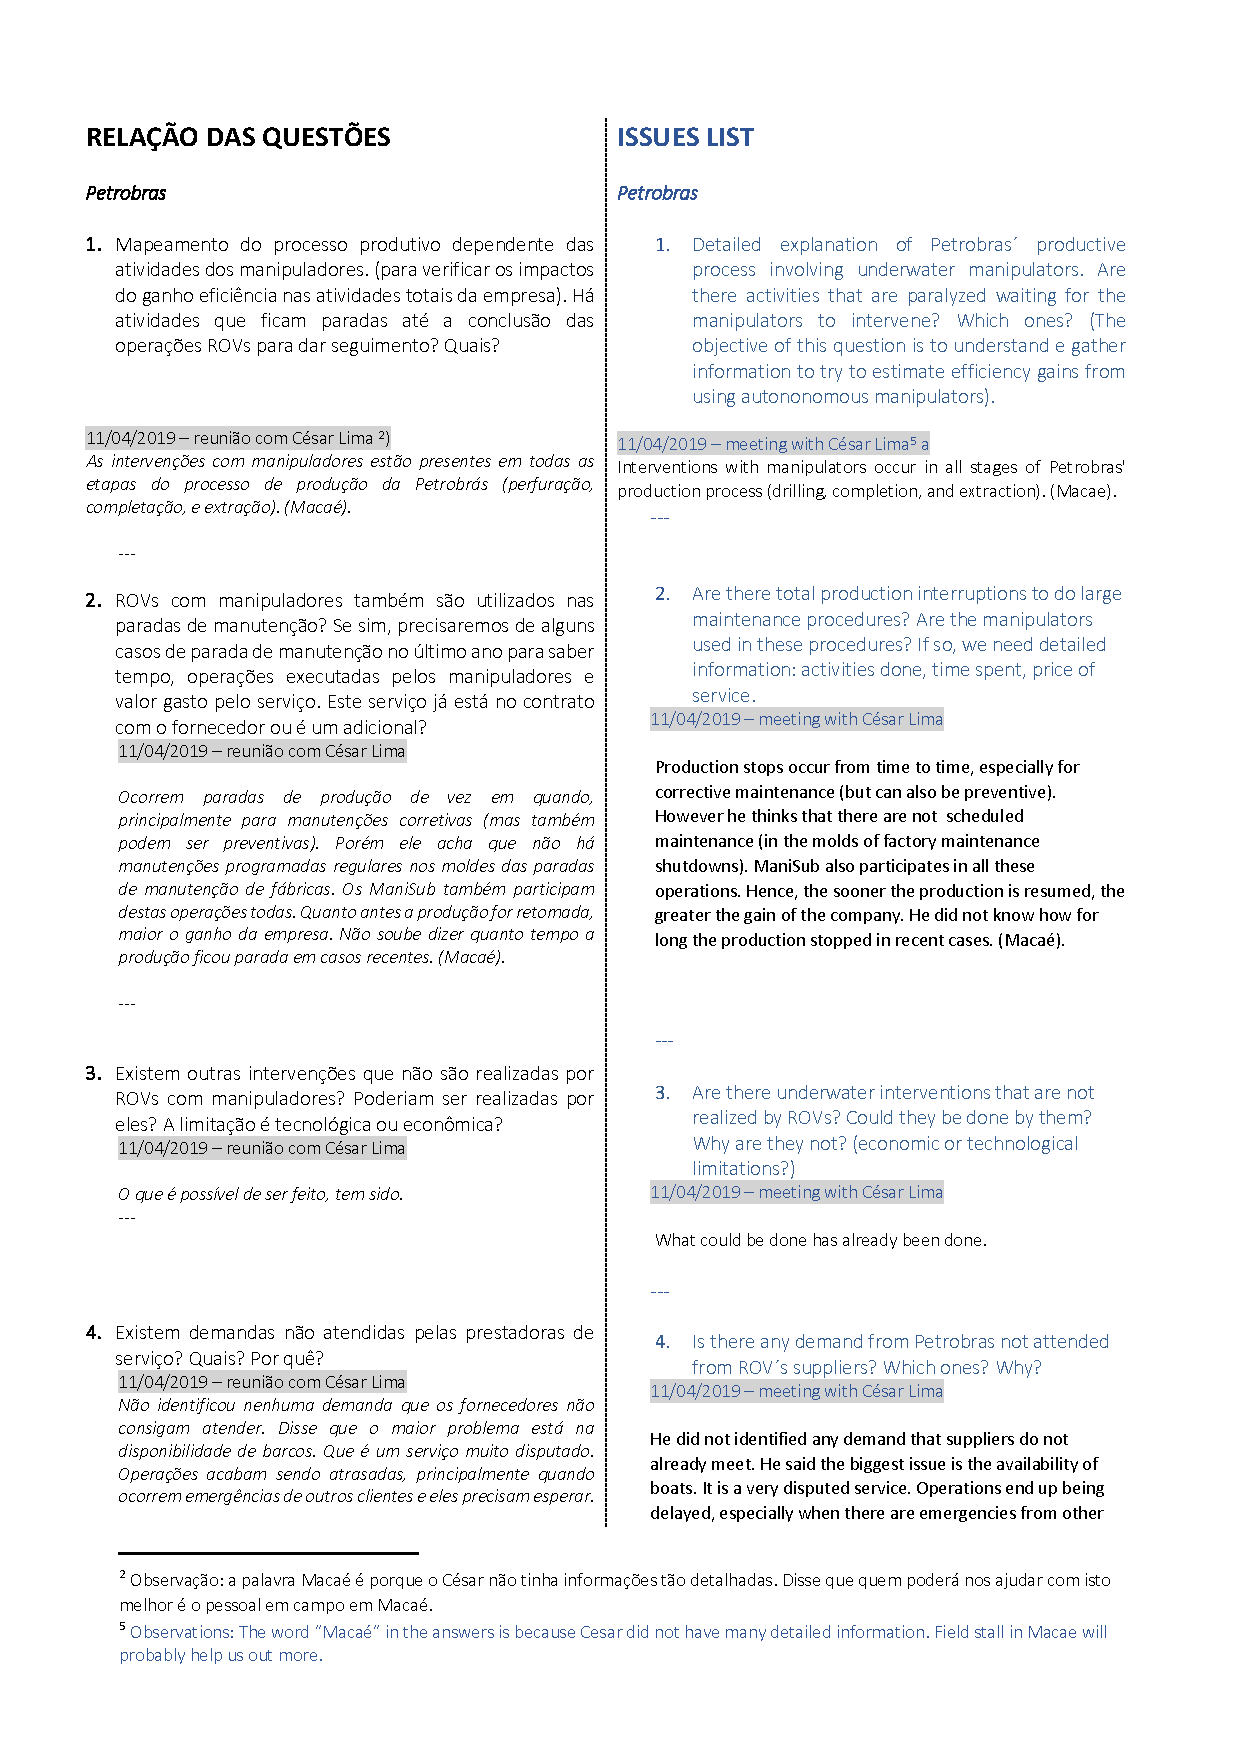
\includepdf[pages={{},-}]{appendix/listquest.pdf}
	%
	%\chapter{Simulação}
	%\lipsum[1] % Comentar e adicionar apêndice aqui
	%
	%\chapter{Prova do Conceito}
	%\includepdf[pages={{},-}]{appendix/poc.pdf}
% --------------------------------------------------------------------------
% Anexos                                                                     
	\anexos
	\justify
	%
	\chapter{Relatório de busca de anterioridade}
	\label{ann:relant}
	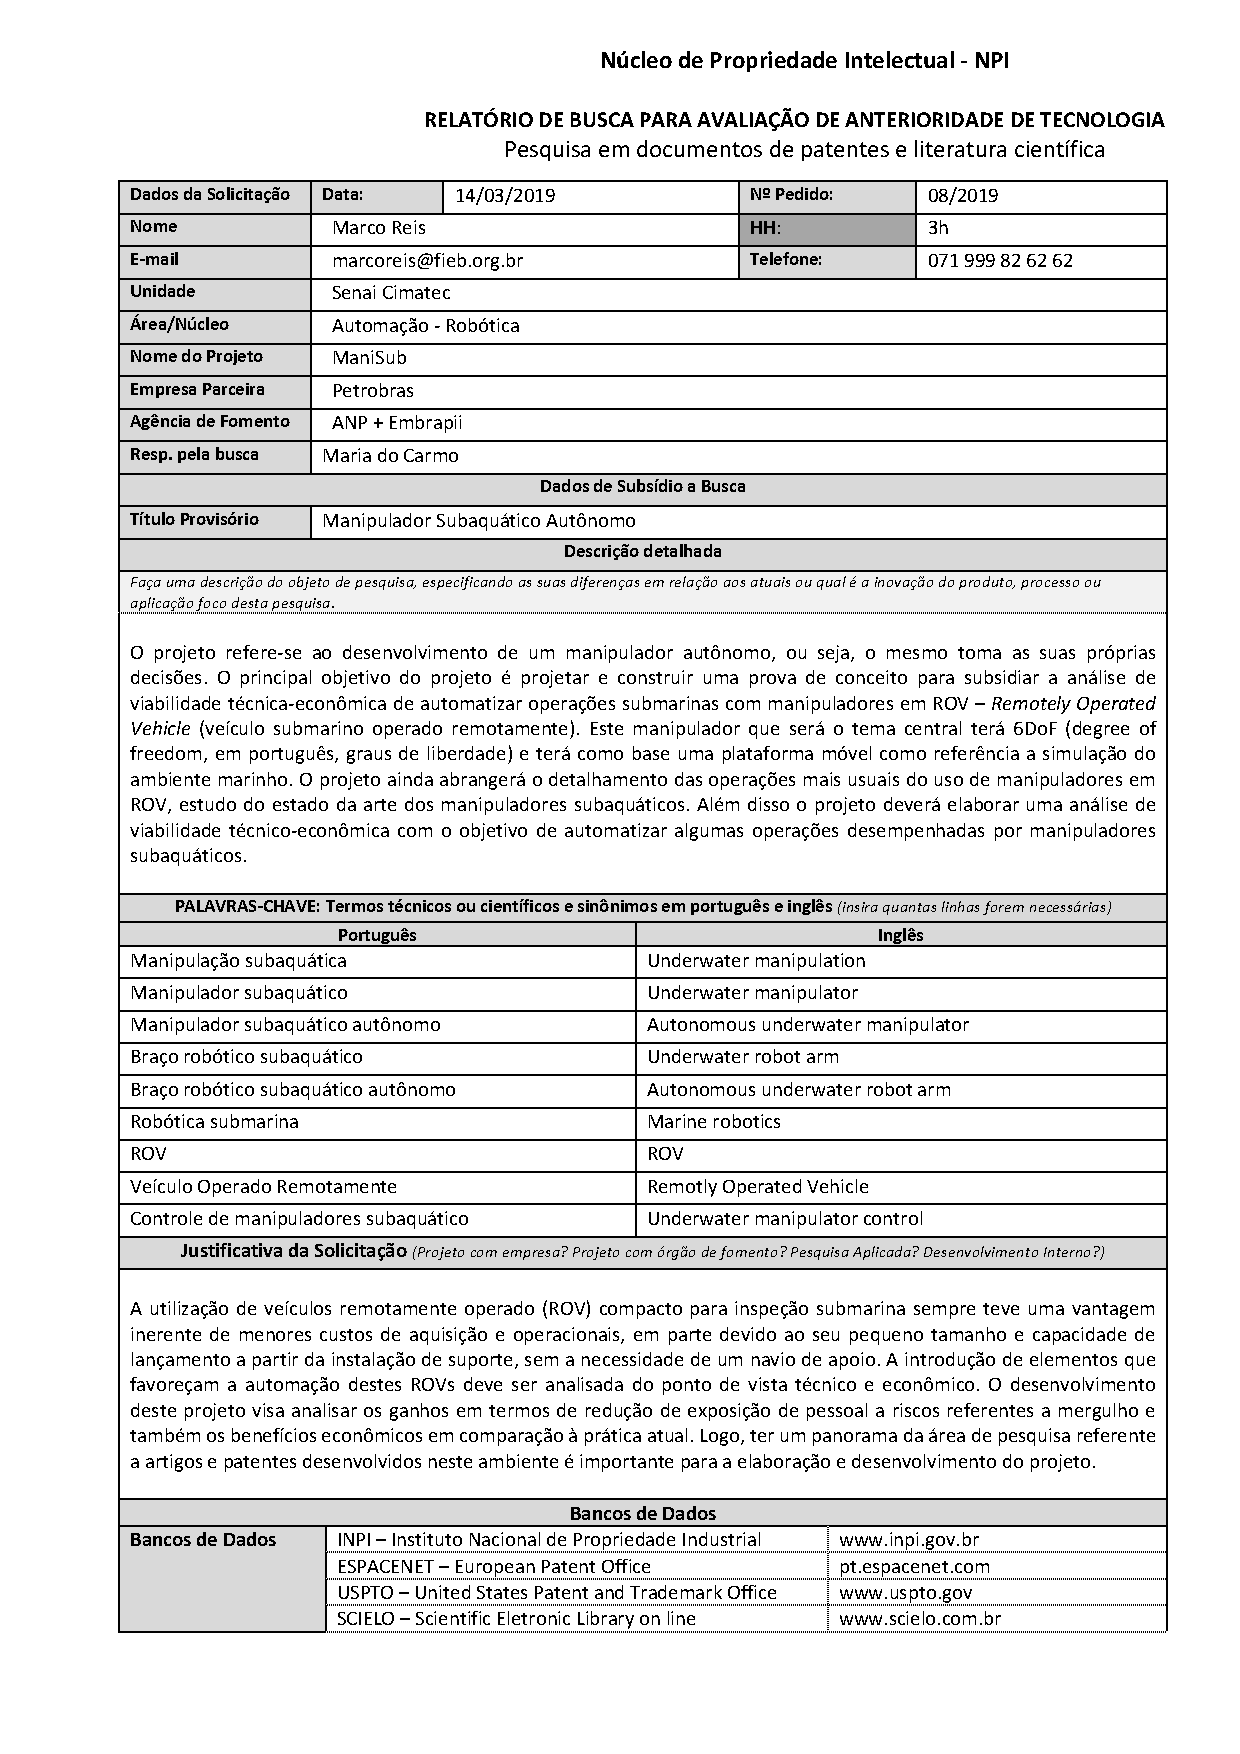
\includepdf[pages={{},-}]{annex/manisubanterioridade.pdf}
	%
\end{document} 